\section{Identifying LCS candidates numerically}
\label{sec:identifying_lcs_candidates_numerically}

\textcite{farazmand2012computing} found
%the identification of the
%zeros of the inner product in~\cref{eq:lcsexistence4}
some of the conditions of \cref{thm:lcsexistence} to be numerically sensitive.
Therefore, they suggest a reformulated set of conditions which make for a more
robust numerical implementation:
\begin{subequations}
    \label{eq:numericalexistence}
    \begin{align}
        \label{eq:numericalexistence1}
        &\lambda_{1}(\vct{x}_{0})\neq\lambda_{2}(\vct{x}_{0})>1,\\
        \label{eq:numericalexistence2}
        &\big\langle\vct{\xi}_{2}(\vct{x}_{0}),%
            \mtrx{H}_{\lambda_{2}}(\vct{x}_{0})%
            \vct{\xi}_{2}(\vct{x}_{0})\big\rangle \leq 0,\\
        \label{eq:numericalexistence3}
        &\vct{\xi}_{1}(\vct{x}_{0})\parallel\mathcal{M}(t_{0}),\\
        \label{eq:numericalexistence4}
        &\begin{gathered}
            \overline{\lambda}_{2},\ \textnormal{the average of}%
            \ \lambda_{2}\ \textnormal{over a curve}\ \gamma,\ %
            \textnormal{is maximal on}\ \mathcal{M}(t_{0})\\ %
            \hspace{-1.3em}\textnormal{among all}\ \textnormal{nearby curves}\ %
            \gamma\ \textnormal{satisfying}\ \gamma\parallel\vct{\xi}_{1}(\vct{x}_{0}).
        \end{gathered}
    \end{align}
\end{subequations}
The relaxation of condition~\eqref{eq:lcsexistence2} in~\cref{thm:lcsexistence}
from strict inequality to condition~\eqref{eq:numericalexistence2}, also
allowing equality, means that LCSs may have finite thickness.
However, the set of criteria given in equation ~\eqref{eq:numericalexistence}
enforce that all LCSs have uniquely defined local orientations. Conditions
\eqref{eq:lcsexistence3} and~\eqref{eq:numericalexistence3} are equivalent,
due to the orthogonality of the eigenvectors $\vct{\xi}_{1}(\vct{x}_{0})$ and
$\vct{\xi}_{2}(\vct{x}_{0})$, although the form~\eqref{eq:numericalexistence3}
turns out to be more advantageous for use in computations. For details
regarding the numerical implementation of conditions
\eqref{eq:numericalexistence3} and~\eqref{eq:numericalexistence4}, see
\cref{sub:a_framework_for_computing_smooth_strainlines}.% for details.

Because of the extension of the main computational grid, as outlined
in \cref{sub:generating_a_set_of_initial_conditions}, the Cauchy-Green strain
tensor could be calculated for the innermost of the padded rows and columns
by means of the same centered difference methods as described in
\cref{sec:calculating_the_cauchy_green_strain_tensor}. Thus, a similar
centered differencing approach was used in order to approximate the Hessian
matrices of the set of eigenvalues $\lambda_{2}(\vct{x}_{0})$ for the main
tracers in the principal grid, that is, the main tracers which originate from
within (or on the borders of) the computational domain
$\mathcal{U}=[0,\hspace{0.5ex}2]\times[0,\hspace{0.5ex}1]$.

\subsection{A framework for computing smooth strainlines}
\label{sub:a_framework_for_computing_smooth_strainlines}

Per condition~\eqref{eq:numericalexistence3}, hyperbolic LCSs are composed
of material curves tangent to the $\vct{\xi}_{1}(\vct{x}_{0})$ vector field,
i.e., the eigenvector field associated with the smaller eigenvalue field
$\lambda_{1}(\vct{x}_{0})$ of the Cauchy-Green strain tensor field
$\mtrx{C}_{t_{0}}^{t}(\vct{x}_{0})$. Traditionally, curves which are
everywhere tangent to the eigenvector field corresponding to the largest
eigenvalues of a two-dimensional tensor field have been called tensor lines
\parencite{farazmand2012computing}. Thus, in order to distinguish between
the tensor lines tangent to $\vct{\xi}_{1}$ and those tangent to
$\vct{\xi}_{2}$, the tensor lines tangent to the $\vct{\xi}_{1}$-field will be
referred to as \emph{strainlines} in the following; a term coined by
\citeauthor{farazmand2012computing}. Aside from
points within $\mathcal{U}$ which exhibit orientational discontinuities in both
eigenvector fields, strainlines can be computed as smooth trajectories of the
ordinary differential equation
\begin{equation}
    \label{eq:strainlinebasicode}
\vct{r}'=\vct{\xi}_{1}(\vct{r}),\quad\vct{r}\in\mathcal{U},%
    \quad\norm{\vct{\xi}_{1}(\vct{r})}=1,
\end{equation}
where, because the eigenvectors $\vct{\xi}_{1}$ are stationary,
the numerical integration is spatial, in principle. However, in order to conform
with the established conventions with regards to the numerical integration of
ODEs, we consider pseudotime --- that is, a ficticious time-like coordinate $s$
is introduced, where advancing $s$ by a numerical integration step $\Delta$
corresponds to a spatial translation by the same length, because the
eigenvectors $\vct{\xi}_{1}$ are normalized to unit length.

As pointed out by \textcite{onu2015lcstool}, the orientational discontinuities
of the $\vct{\xi}_{1}$-field are removable, through careful monitoring and
local reorientation. This process is illustrated in figure
\ref{fig:locallinearinterp}, and can be described in terms of three steps.
First, the four nearest neighboring grid points to $\vct{r}$ are identified.
Then, orientational discontinuities inbetween the grid elements are found
by inspecting the inner product of the $\vct{\xi}_{1}$ vectors of adjacent grid
points. Rotations exceeding $90\si{\degree}$ between pairs of neighboring
vectors are labelled as orientational discontinuities. These are corrected
prior to linear interpolation by flipping the corresponding vectors by
$180\si{\degree}$. In the end, linear interpolation is used within the grid
element whose corners are defined by the four nearest neighbors to $\vct{r}$.

Furthermore, should the $\vct{\xi}_{1}$-vector obtained from the local
special-purpose linear interpolation outlined above prove to be rotated by more
than $90\si{\degree}$ relative to the interpolated $\vct{\xi}_{1}$-vector
at the previous point of the strainline, it would be flipped $180\si{\degree}$,
to facilitate smooth trajectories through oriental discontinuities.
The entire process of this special-purpose local linear interpolation method is
outlined in figure~\ref{fig:locallinearinterp}.

\begin{figure}[htpb]
    \centering
    \def\svgwidth{0.8\linewidth}
    \begin{figure}[htpb]
    \centering
    \def\svgwidth{0.8\linewidth}
    \begin{figure}[htpb]
    \centering
    \def\svgwidth{0.8\linewidth}
    \input{figures/linearspecialinterp.pdf_tex}
    \caption[Illustration of the special linear interpolation used
    for the $\vct{\xi}_{1}$ eigenvector field]
    {Illustration of the special-purpose linear interpolation used to compute
        trajectories of the $\vct{\xi}_{1}$ eigenvector field. At point
        \textbf{(a)}, there is an orientational discontinuity at the lower
        right grid point, which is corrected by rotating the corresponding
        vector by $180\si{\degree}$ prior to linear interpolation. At point
        \textbf{(b)}, there is no orientational discontinuity. Lastly,
        at point \textbf{(c)}, the interpolated vector must be flipped due
    to the overall orientation of the trajectory.}
    \label{fig:locallinearinterp}
\end{figure}

    \caption[Illustration of the special linear interpolation used
    for the $\vct{\xi}_{1}$ eigenvector field]
    {Illustration of the special-purpose linear interpolation used to compute
        trajectories of the $\vct{\xi}_{1}$ eigenvector field. At point
        \textbf{(a)}, there is an orientational discontinuity at the lower
        right grid point, which is corrected by rotating the corresponding
        vector by $180\si{\degree}$ prior to linear interpolation. At point
        \textbf{(b)}, there is no orientational discontinuity. Lastly,
        at point \textbf{(c)}, the interpolated vector must be flipped due
    to the overall orientation of the trajectory.}
    \label{fig:locallinearinterp}
\end{figure}

    \caption[Illustration of the special linear interpolation used
    for the $\vct{\xi}_{1}$ eigenvector field]
    {Illustration of the special-purpose linear interpolation used to compute
        trajectories of the $\vct{\xi}_{1}$ eigenvector field. At point
        \textbf{(a)}, there is an orientational discontinuity at the lower
        right grid point, which is corrected by rotating the corresponding
        vector by $180\si{\degree}$ prior to linear interpolation. At point
        \textbf{(b)}, there is no orientational discontinuity. Lastly,
        at point \textbf{(c)}, the interpolated vector must be flipped due
    to the overall orientation of the trajectory.}
    \label{fig:locallinearinterp}
\end{figure}


So, in order to compute globally smooth strainlines,
\cref{eq:strainlinebasicode} is altered in the following way:
\begin{equation}
    \label{eq:strainlineode}
    \vct{r}'(s)= \vct{f}\big(\vct{r}(s)\big),
\end{equation}
where $\vct{f}$ denotes the special-purpose local linear interpolation of
the $\vct{\xi}_{1}$ field, as outlined above and in figure
\ref{fig:locallinearinterp}.
%, and $\Delta$ is the numerical pseudotime step
% length used in the numerical integration.
%while the signum function is defined as
%\begin{equation}
%    \label{eq:signumfunction}
%\sgn(x)=\begin{cases}1,&\textnormal{for}\ x>0\\
%        0,&\textnormal{for}\ x=0\\
%        -1,&\textnormal{for}\ x<0\end{cases}
%\end{equation}

\subsection{Extracting hyperbolic LCSs from strainlines}
\label{sub:extracting_hyperbolic_lcss_from_strainlines}

If a material line $\mathcal{M}(t_{0})$ lies within a strainline, it
automatically fulfills condition~\eqref{eq:numericalexistence3},
as a trajectory of the $\vct{\xi}_{1}$-field is, per definition, always
parallel to it. The segments of the strainlines on which the remaining
conditions~\eqref{eq:numericalexistence1},~\eqref{eq:numericalexistence2} and
\eqref{eq:numericalexistence4} are satisfied comprises the set of hyperbolic
LCSs in the flow over time interval $[t_{0},t_{0}+T]$.
\textcite{farazmand2012computing} suggest that in order to identify this
set of LCSs, one should start by identifying the subdomain
$\mathcal{U}_{0}\subset\mathcal{U}$ on which the conditions
\eqref{eq:numericalexistence1} and~\eqref{eq:numericalexistence2} are satisfied,
and then integrate the system given by equation~\eqref{eq:strainlineode} from
initial conditions within $\mathcal{U}_{0}$ to construct strainlines.
Generally, the integration proceeds until each strainline reaches the domain
boundaries of $\mathcal{U}$, or reaches a degenerate point (see below) of the
original $\vct{\xi}_{1}$ vector field.

Using all of the points in the $\mathcal{U}_{0}$ domain would inevitably
involve computing a lot of strainlines several times over. In order to
reduce the number of redundant calculations, the set of considered strain
initial conditions were reduced, with the approach suggested by
\textcite{farazmand2012computing}. In particular, the set $\mathcal{U}_{0}$
was reduced to its intersections with four horizontal and four vertical lines.
The set $\mathcal{U}_{0}$ for the double gyre system, as well as the
aforementioned intersections, are illustrated in figure~\ref{fig:u0_domain}.
The reduced set of strain initial conditions consists of 1470 grid points, which
is two orders of magnitude less than the total number of points in
$\mathcal{U}_{0}$.

\begin{figure}[htpb]
    \centering
    \begin{subfigure}{\textwidth}
        \centering
        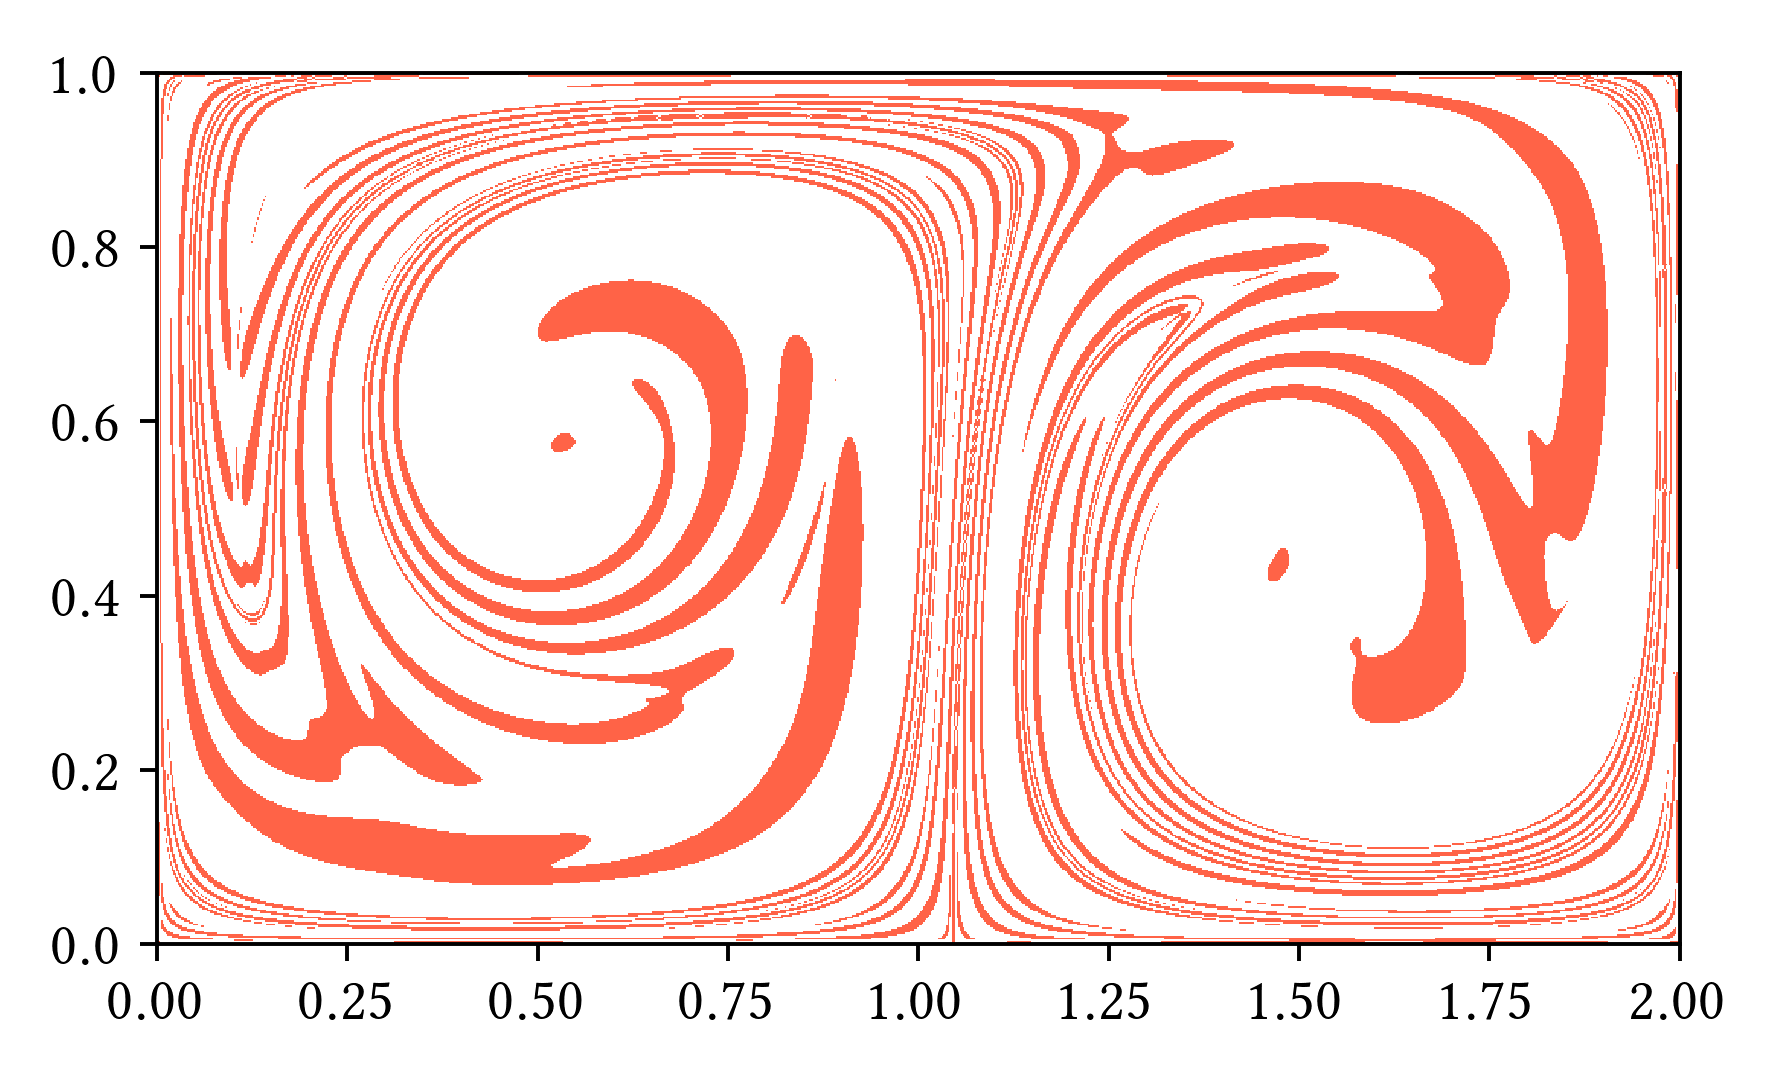
\includegraphics{figures/domain_figures/u0_dom.png}
%        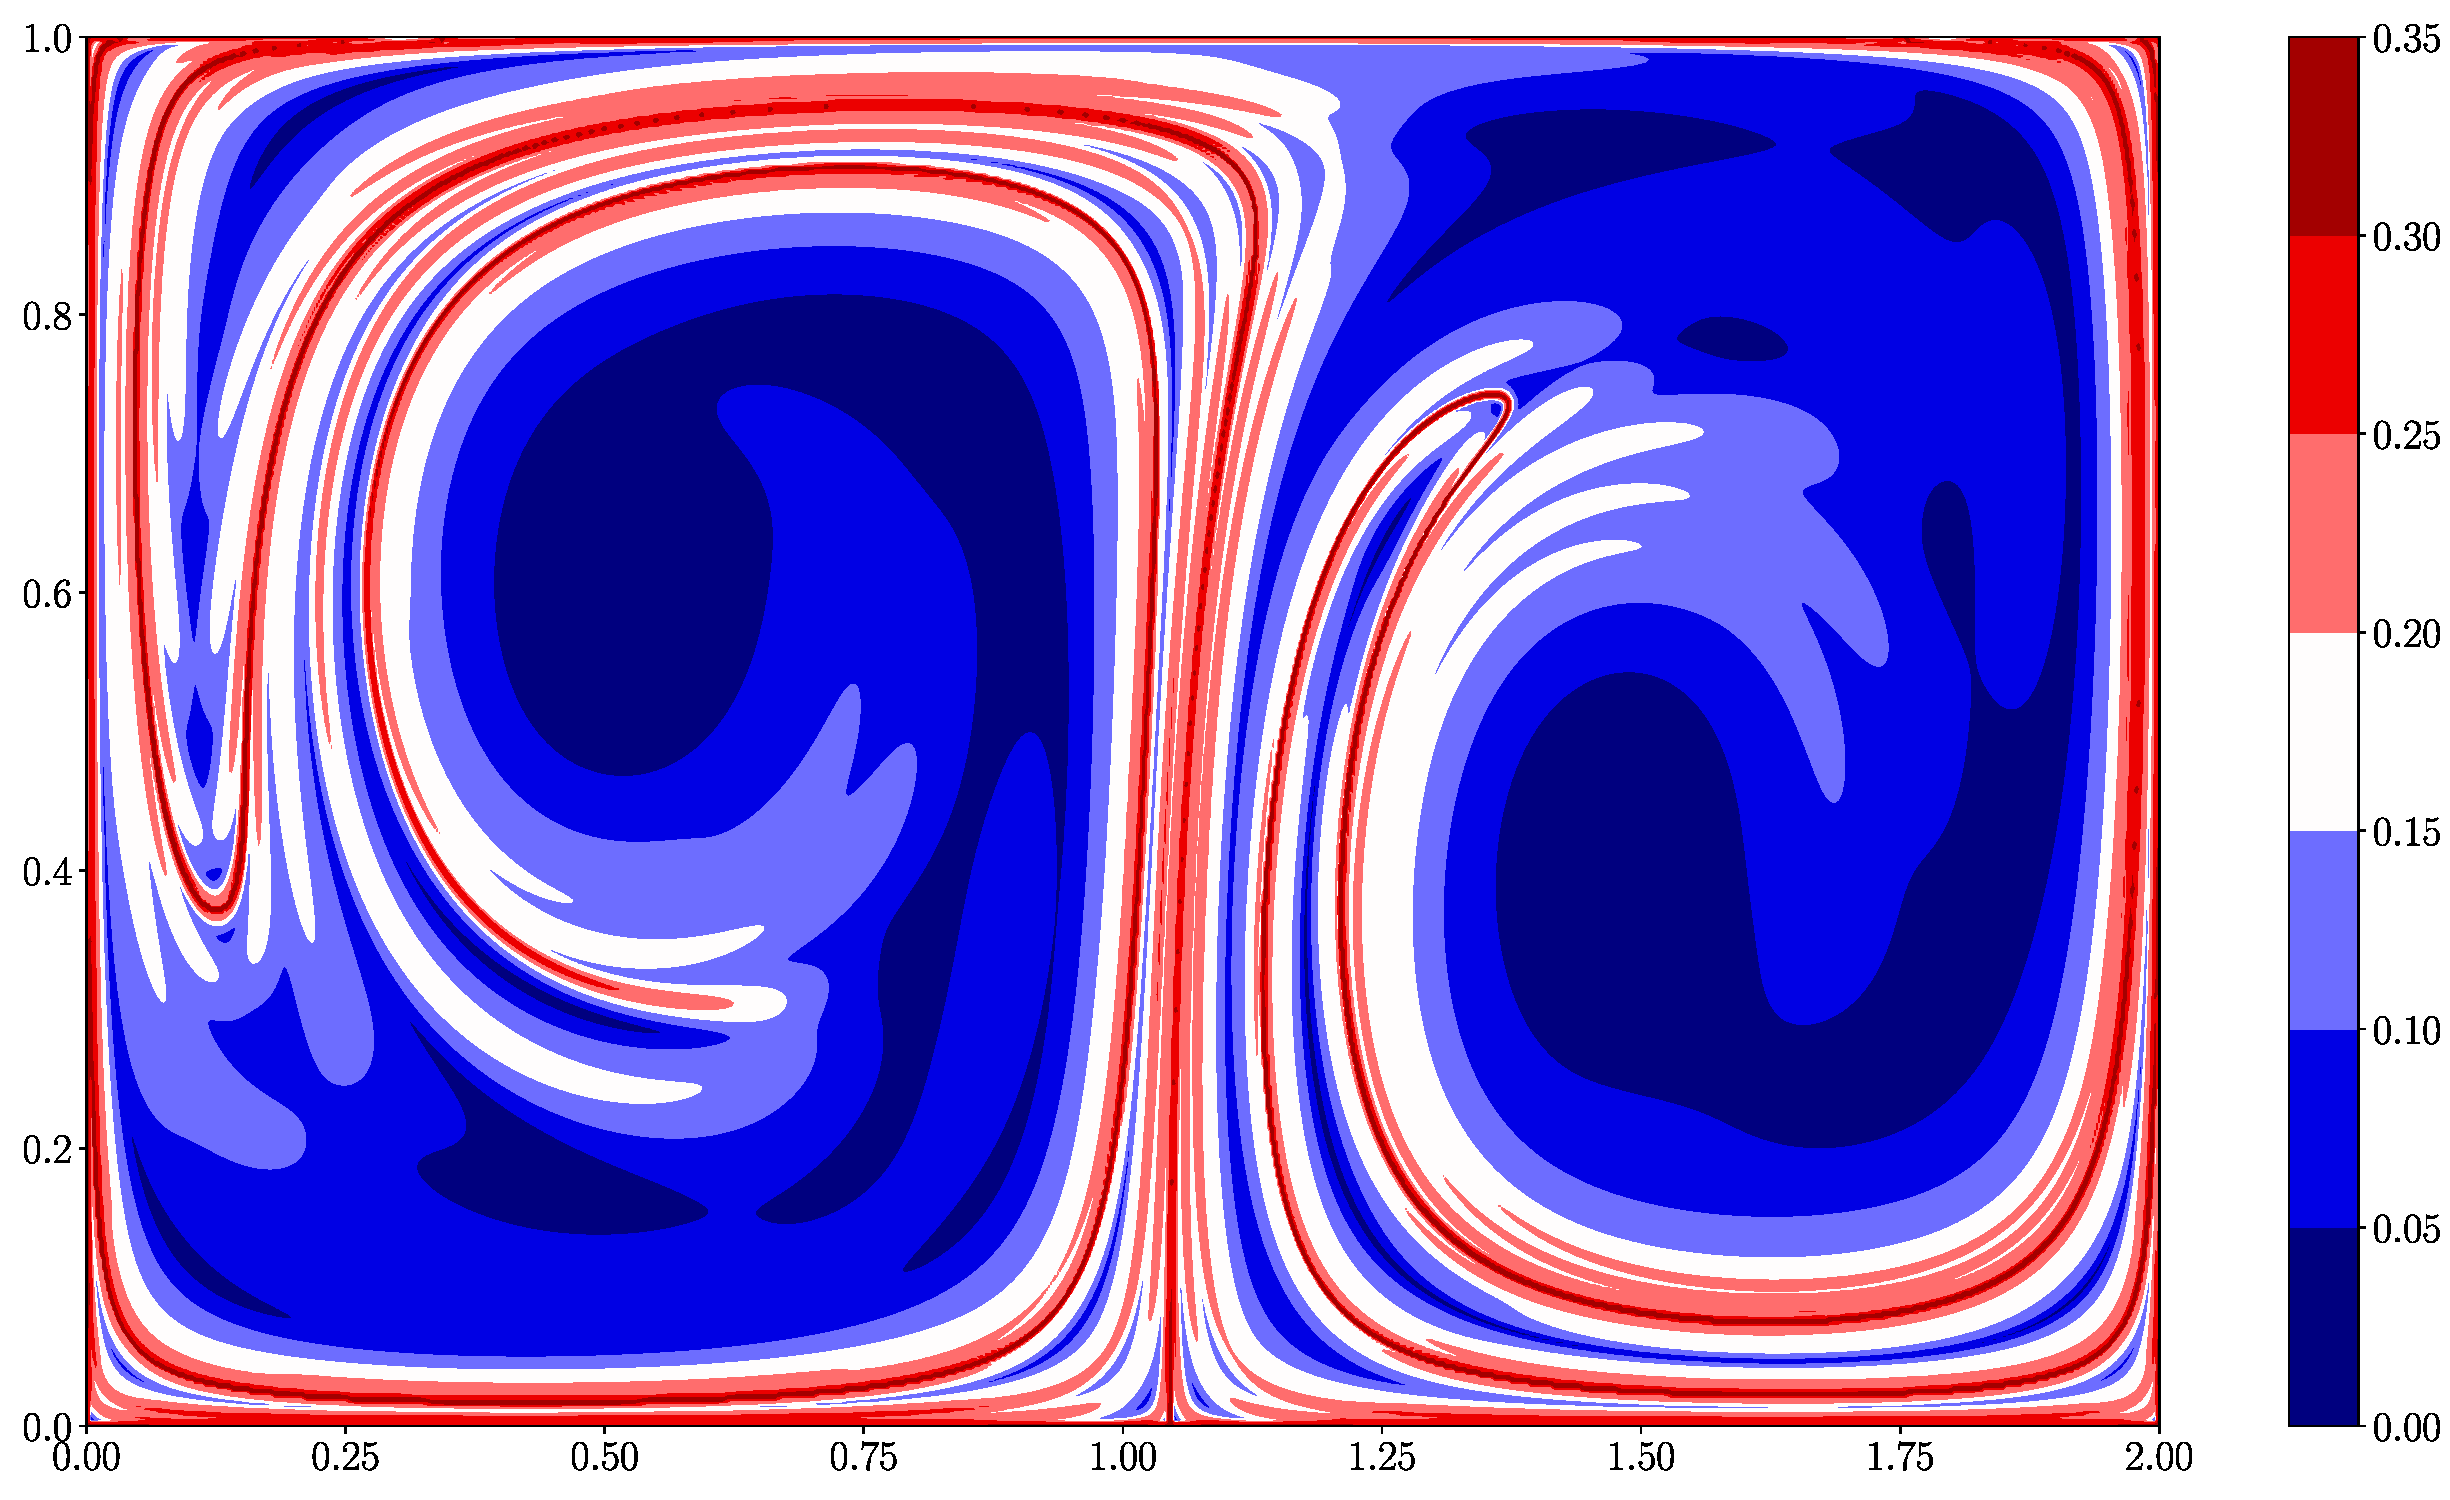
\includegraphics[width=0.75\linewidth,keepaspectratio]{figures/ftle.pdf}
    \end{subfigure}

    \begin{subfigure}{\textwidth}
        \centering
        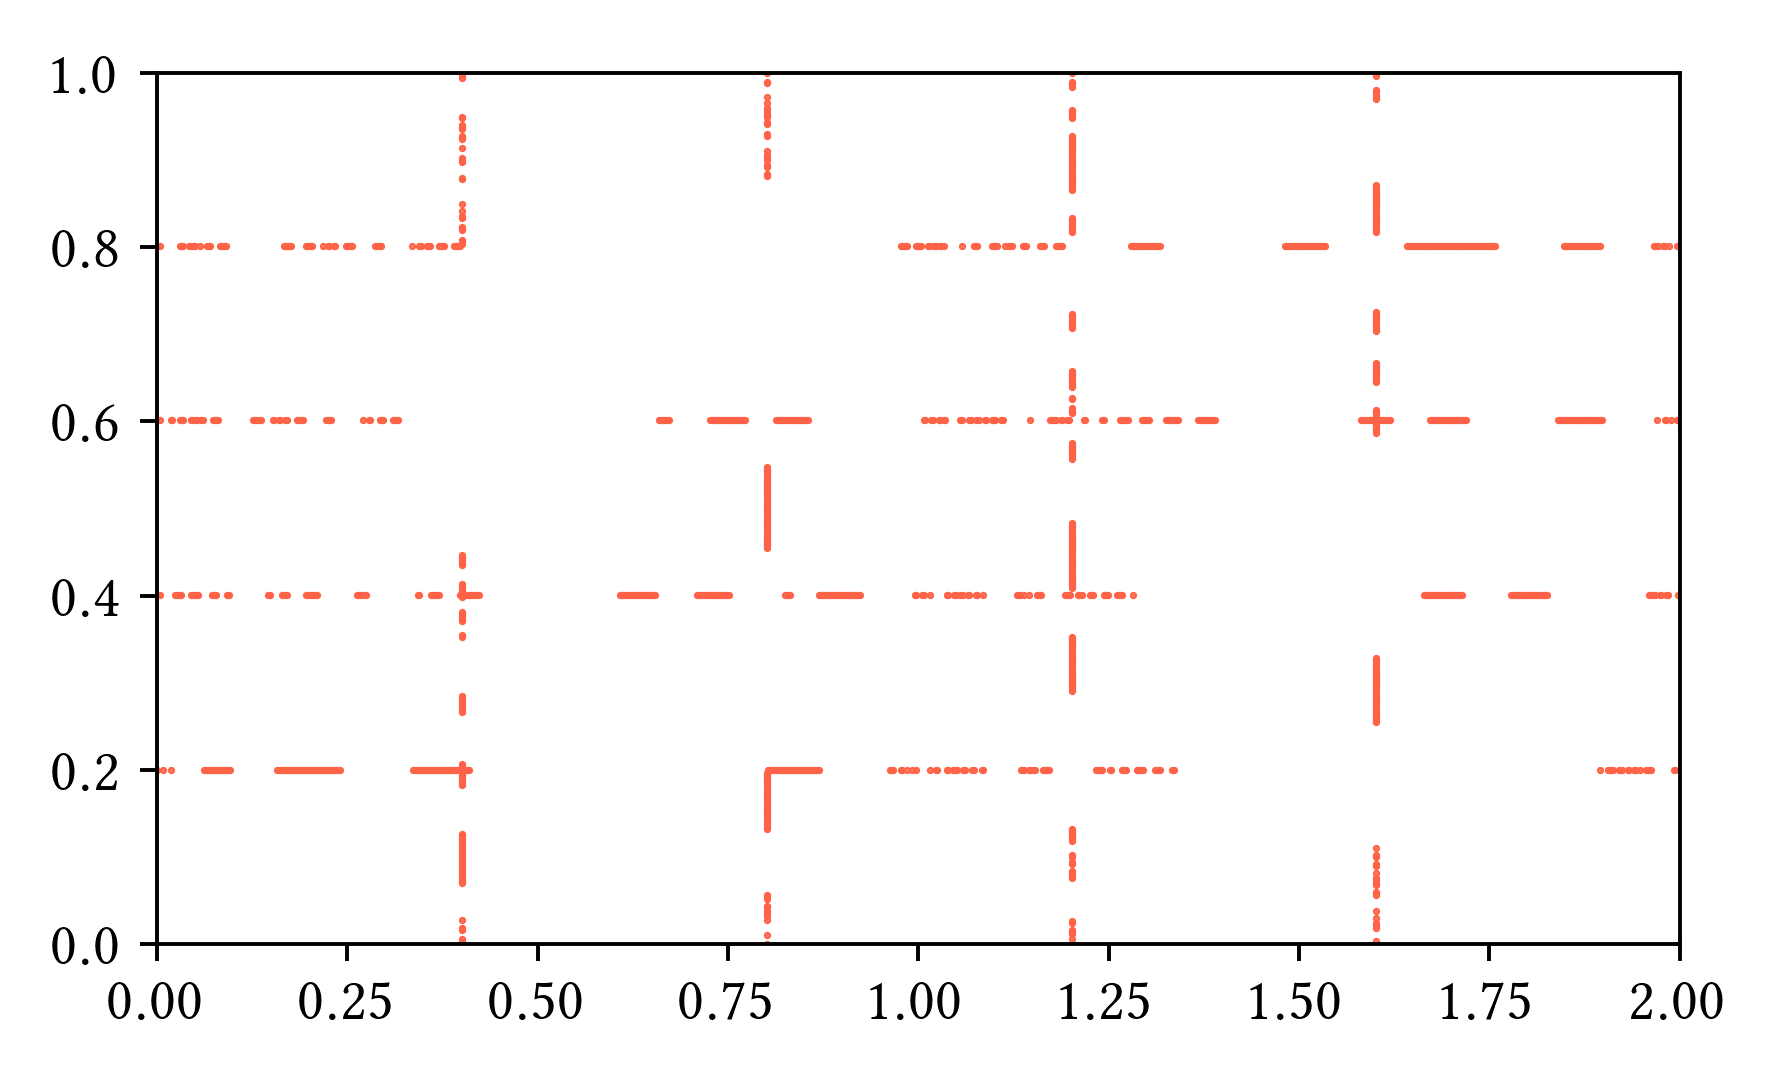
\includegraphics{figures/domain_figures/g0_dom.png}
%        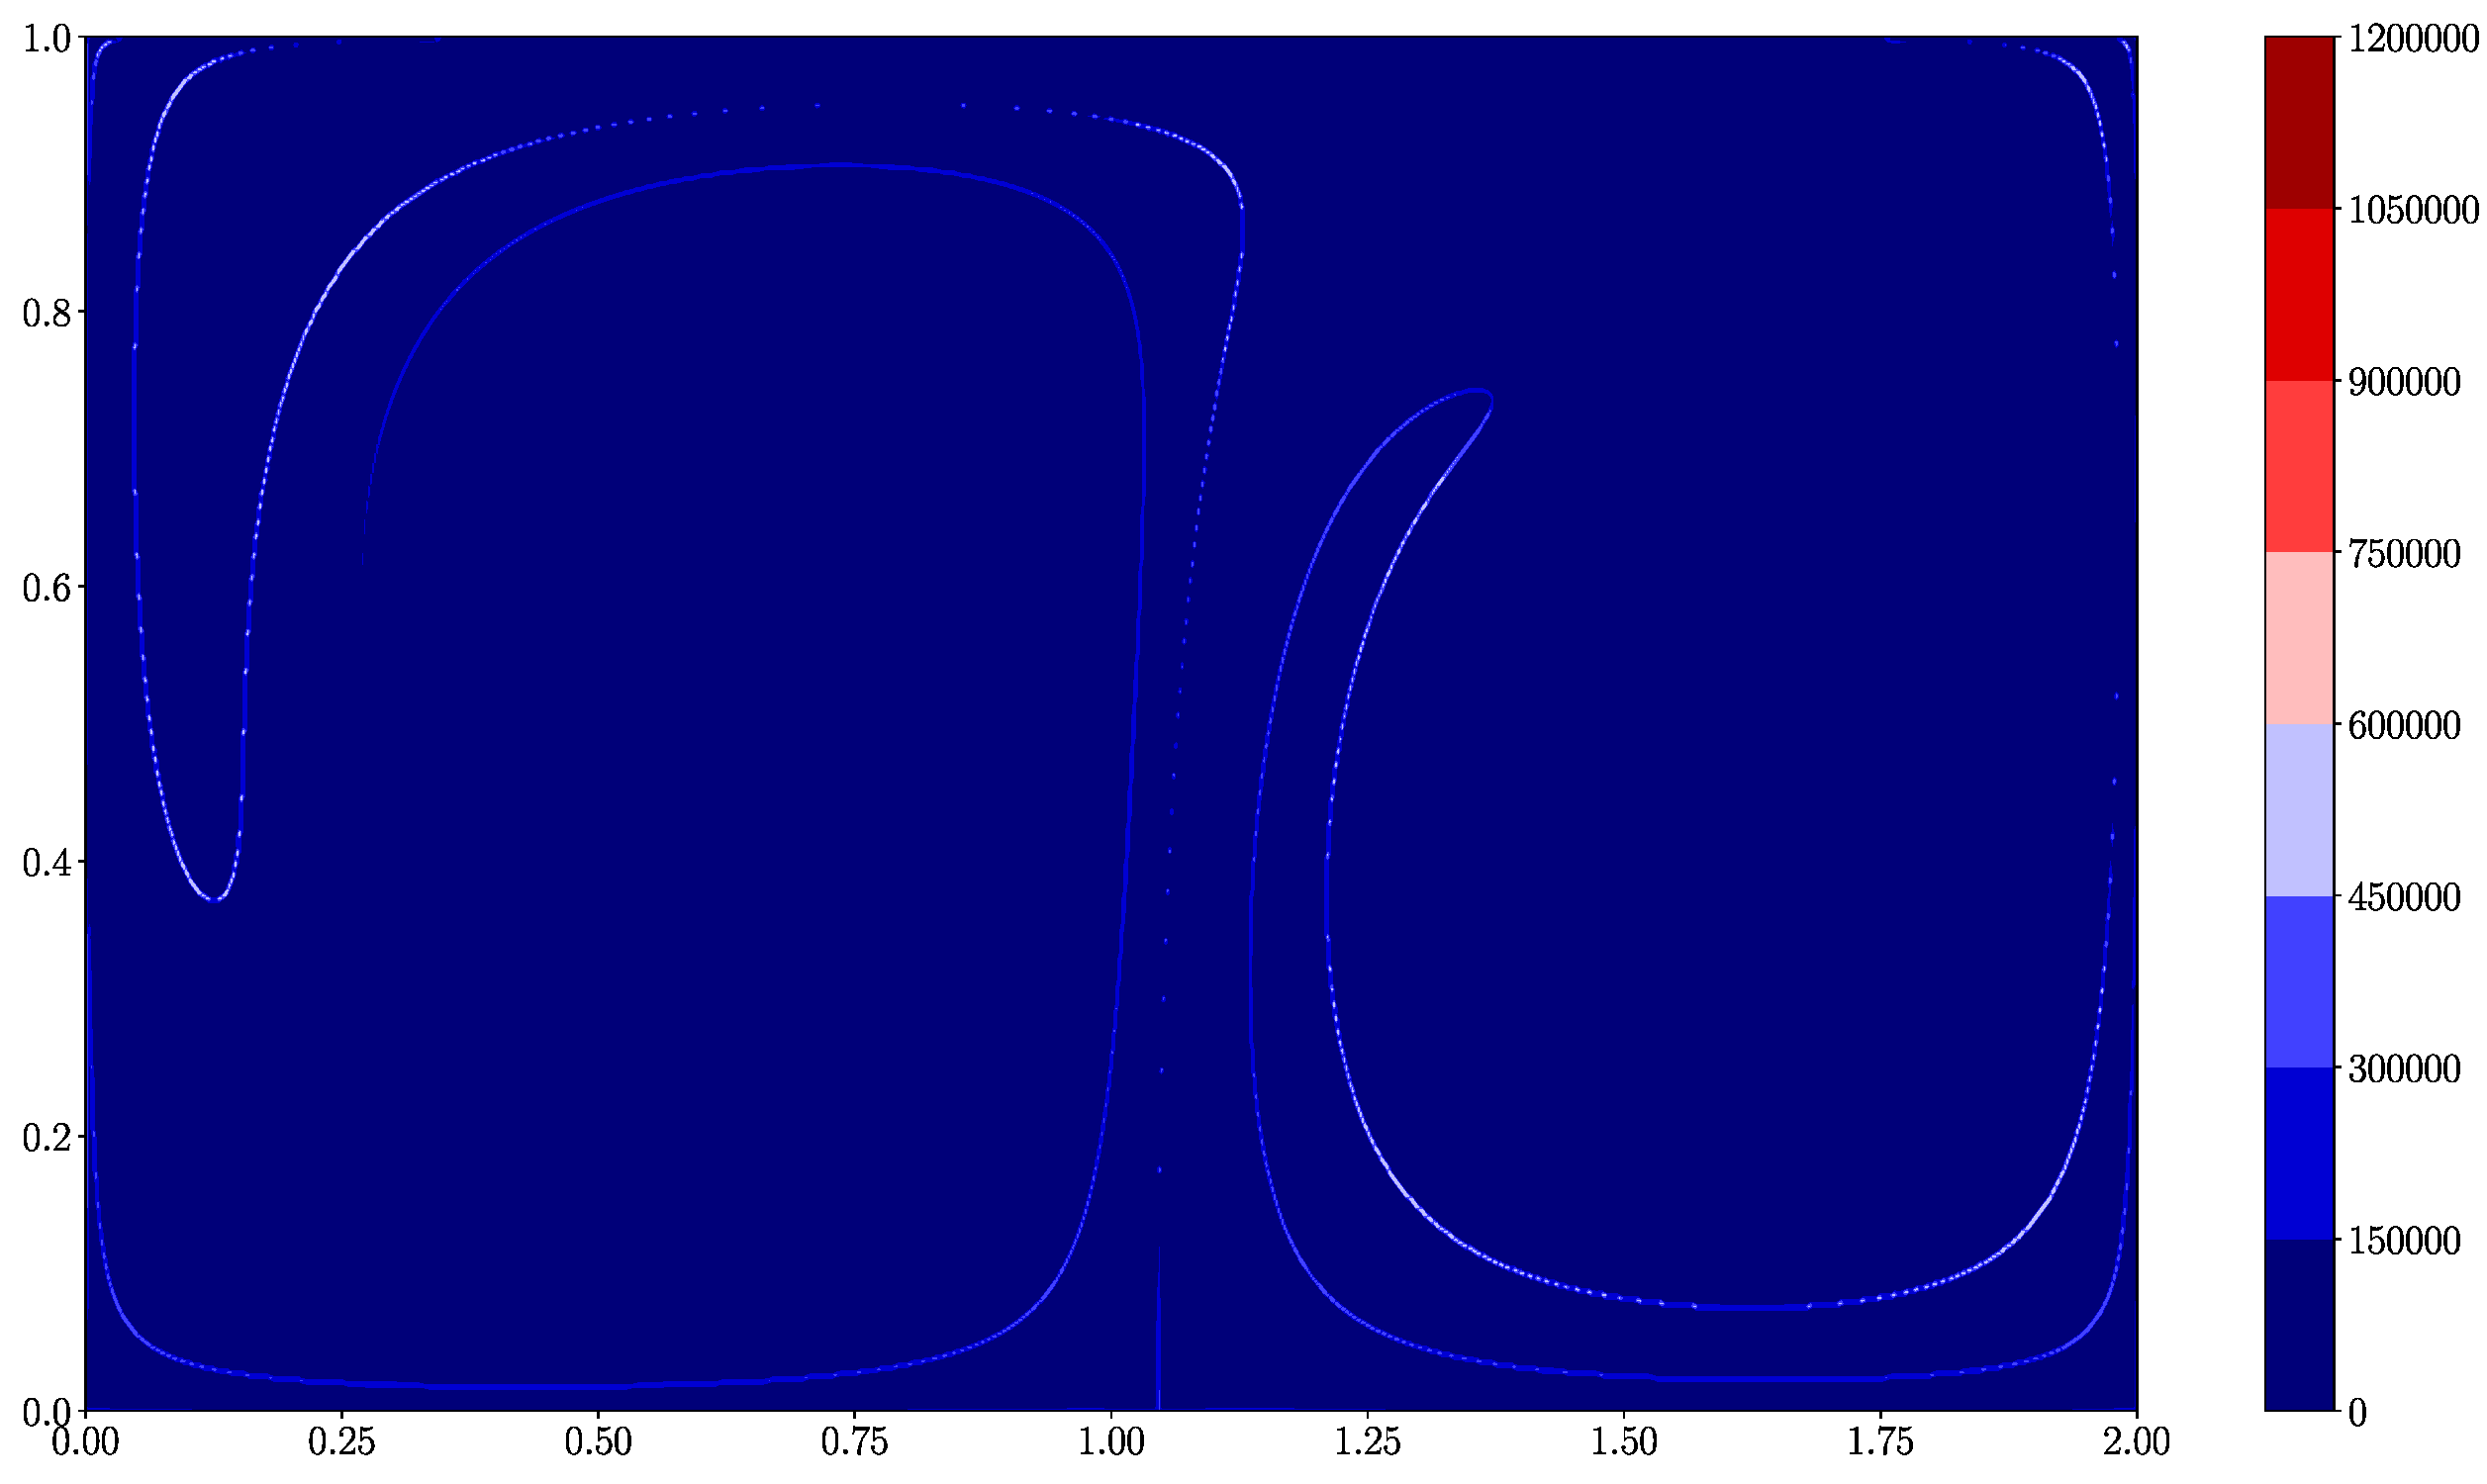
\includegraphics[width=0.75\linewidth,keepaspectratio]{figures/lambda2.pdf}
    \end{subfigure}
    \caption[The set $\mathcal{U}_{0}$ for the double gyre system, and the
    reduced set of strain initial conditions]{The set
        $\mathcal{U}_{0}$ for the double gyre system, given by
    \cref{eq:doublegyre,eq:doublegyrefuns,eq:doublegyreparams}, is shown at the
    top. This is the set of initial conditions where the LCS existence
    conditions given in \cref{eq:numericalexistence1,eq:numericalexistence2}
    are satisfied.  Its intersection with a set of four horizontal and four
    vertical, equidistant lines is shown at the bottom. The latter was used as
    the set of strain initial conditions, in order to eliminate (or at least,
    reduce the amount of) redundant computations of strainlines within
$\mathcal{U}_{0}$.}
    \label{fig:u0_domain}
\end{figure}

%\clearpage
The degenerate points of the $\vct{\xi}_{1}$ vector field is, as the name
implies, the set of points in $\mathcal{U}$ for which the eigenvalues
$\lambda_{1}(\vct{x}_{0})$ and $\lambda_{2}(\vct{x}_{0})$ are equal, leaving
the strain eigenvector field $\vct{\xi}_{1}$ undefined. As a computational
measure of this degeneracy, the scalar field defined as
\begin{equation}
    \label{eq:alphafield}
    \alpha(\vct{x}_{0})=\bigg(\dfrac{%
                        \lambda_{2}(\vct{x}_{0})-\lambda_{1}(\vct{x}_{0})}%
                    {\lambda_{2}(\vct{x}_{0})+\lambda_{1}(\vct{x}_{0})}\bigg)^{2}
\end{equation}
was used, inspired by~\textcite{farazmand2012computing}. For points $\vct{x}$
which did not coincide with the grid points $\vct{x}_{i,j}$, the values
$\lambda_{1}(\vct{x})$ and $\lambda_{2}(\vct{x})$ were found by means of
regular linear interpolation. Wherever the value of $\alpha(\vct{x})$ decreased
below a predefined threshold of $10^{-6}$, the point $\vct{x}$ was flagged as
degenerate, thus stopping the strainline integration.

Generally, one expects the selected strain initial conditions, shown in figure
\ref{fig:u0_domain}, to be located somewhere in the middle of a strainline.
Hence, two strainline segments were computed
and merged for each initial condition; one moving forwards in pseudotime, and
one moving backwards, i.e., using the $180\si{\degree}$ rotated
$\vct{\xi}_{1}$ vector field in the system given by \cref{eq:strainlineode}.
This ensured that no strainline was ended prematurely, purely as a consequence
of the reduced number of strain initial conditions. Furthermore, the classical
Runge-Kutta method with an integration step length $\Delta=10^{-3}$ was used in
order to compute all of the strainlines, regardless of the integration scheme
used in the advection of the tracers, described in
\cref{sec:advecting_a_set_of_initial_conditions}. The classical Runge-Kutta
method was applied universally for consistency, and chosen for its simplicity
and relative accuracy. Moreover, this project is centered around the dependence
of the choice of integration method in the tracer advection. The step length was
made to be half of the main grid spacing, to ensure that the micro-scale strain
behaviour would be encapsulated in the resulting strainlines, while maintaining
reasonable computation times.
%presented in
%\cref{sub:on_the_choice_of_numerical_step_lengths_and_tolerance_levels};
%however, there is no way of knowing in advance, how long (in terms of numerical
%integration steps) any given strainline will be. For this reason, it is
%impossible to estimate the accumulated floating-point arithmetic errors in
%advance. Regardless, we expect diminishing returns in terms of numerical
%accuracy by lowering the step length even further, because the accuracy is
%always bounded from below by the inherent accuracy of the double-precision
%floating-point numbers.

Frequently, only a segment of any given strainline will qualify as a hyperbolic
LCS\@. Hence, the integration of any strainline can be stopped when it reaches
a point at which one of the conditions~\eqref{eq:numericalexistence1} or
\eqref{eq:numericalexistence2} fails. Doing so uncritically, however, opens up
the possibility of stopping a strainline which only exited the $\mathcal{U}_{0}$
domain due to numerical noise. In order to avoid such unwanted failures,
the approach of \textcite{farazmand2012computing} was followed.
Therefore, strainline integration was only stopped if one of the aforementioned
LCS conditions fail repeatedly over a pre-set length $l_{\textnormal{f}}=0.2$ of
the strainline. Furthermore, the strainlines which were stopped because
of continuous failure of LCS conditions were cut such that their \emph{new}
endpoints in either direction, as seen from the strain initial condition, were
the last point on which the \emph{original} strainline satisfied the
aforementioned conditions. This concept is illustrated in
\cref{fig:tailcutting}.

\begin{figure}[htpb]
    \centering
    \def\svgwidth{0.8\linewidth}
    \begin{figure}[htpb]
    \centering
    \def\svgwidth{0.8\linewidth}
    \begin{figure}[htpb]
    \centering
    \def\svgwidth{0.8\linewidth}
    \input{figures/tailcutting.pdf_tex}
    \caption[Illustration of the concept of strainline tail end cutting]%
    {Illustration of the concept of strainline tail end cutting. The
    filled, gray ellipsis constitutes a fictitious set of points $\mathcal{U}_{0}$,
    for which the LCS existence conditions expressed in equations
    \eqref{eq:numericalexistence1} and~\eqref{eq:numericalexistence2} hold. A
    strainline, starting at (a), is integrated in both directions in
    pseudotime. In both directions, the strainline integration is eventually
    stopped due to repeated failure of at least one of the two aforementioned
    LCS existence conditions, over a pre-set length $l_{\textnormal{f}}=0.2$.
    The tails at either end, i.e., the parts of the strainline which exited
    the $\mathcal{U}_{0}$ and did not return, are indicated by dashed curves at
    (b) and (c). These were cut, leaving the solid curve as the part of
    the strainline which was considered as an LCS candidate. Although parts
    of \emph{this} curve may reside outside of the $\mathcal{U}_{0}$ domain, these segments are all
\emph{shorter} than $l_{\textnormal{f}}$.}
    \label{fig:tailcutting}
\end{figure}

    \caption[Illustration of the concept of strainline tail end cutting]%
    {Illustration of the concept of strainline tail end cutting. The
    filled, gray ellipsis constitutes a fictitious set of points $\mathcal{U}_{0}$,
    for which the LCS existence conditions expressed in equations
    \eqref{eq:numericalexistence1} and~\eqref{eq:numericalexistence2} hold. A
    strainline, starting at (a), is integrated in both directions in
    pseudotime. In both directions, the strainline integration is eventually
    stopped due to repeated failure of at least one of the two aforementioned
    LCS existence conditions, over a pre-set length $l_{\textnormal{f}}=0.2$.
    The tails at either end, i.e., the parts of the strainline which exited
    the $\mathcal{U}_{0}$ and did not return, are indicated by dashed curves at
    (b) and (c). These were cut, leaving the solid curve as the part of
    the strainline which was considered as an LCS candidate. Although parts
    of \emph{this} curve may reside outside of the $\mathcal{U}_{0}$ domain, these segments are all
\emph{shorter} than $l_{\textnormal{f}}$.}
    \label{fig:tailcutting}
\end{figure}

    \caption[Illustration of the concept of strainline tail end cutting]%
    {Illustration of the concept of strainline tail end cutting. The
    filled, gray ellipsis constitutes a fictitious set of points $\mathcal{U}_{0}$,
    for which the LCS existence conditions expressed in equations
    \eqref{eq:numericalexistence1} and~\eqref{eq:numericalexistence2} hold. A
    strainline, starting at (a), is integrated in both directions in
    pseudotime. In both directions, the strainline integration is eventually
    stopped due to repeated failure of at least one of the two aforementioned
    LCS existence conditions, over a pre-set length $l_{\textnormal{f}}=0.2$.
    The tails at either end, i.e., the parts of the strainline which exited
    the $\mathcal{U}_{0}$ and did not return, are indicated by dashed curves at
    (b) and (c). These were cut, leaving the solid curve as the part of
    the strainline which was considered as an LCS candidate. Although parts
    of \emph{this} curve may reside outside of the $\mathcal{U}_{0}$ domain, these segments are all
\emph{shorter} than $l_{\textnormal{f}}$.}
    \label{fig:tailcutting}
\end{figure}


\clearpage
\subsubsection{Identifying strainlines which are local strain maximizers}
\label{ssub:identifying_strainlines_which_are_local_strain_maximizers}

Now, having located the strainline pieces which satisfy conditions
\eqref{eq:numericalexistence1} and~\eqref{eq:numericalexistence2}, the next
step is imposing condition~\eqref{eq:numericalexistence4}, i.e., identifying the
strainline segments that are local maxima of the averaged maximum strain. In
the following, we let $\{\gamma_{j}\}$ denote the set of parametrized strainline
curves, computed as solutions of the strain ODE system given in
\cref{eq:strainlineode}. The suggested approach of
\textcite{farazmand2012computing} is to define a set $\mathcal{L}$ of uniformly
spaced horizontal and vertical lines within the domain $\mathcal{U}_{0}$. Then,
the values of $\overline{\lambda}_{2}(\gamma_{0})$ --- the average of
$\lambda_{2}$ on the curve $\gamma_{0}$ --- are compared at the neighboring
intersections of all sufficiently close strainline segments along each of the
lines modeline $\mathcal{L}$. The process is illustrated in
\cref{fig:neighborlcs}.

\begin{figure}[htpb]
    \centering
    \def\svgwidth{0.8\linewidth}
    \begin{figure}[htpb]
    \centering
    \def\svgwidth{0.8\linewidth}
    \begin{figure}[htpb]
    \centering
    \def\svgwidth{0.8\linewidth}
    \input{figures/neighborlcs.pdf_tex}
    \caption[The identification process of strainlines which
    are local strain maximizers]{Illustration of the identification process of
        strainlines which are local strain maximizers.
        Local maxima of $\overline{\lambda}_{2}(\gamma)$, the average of
        $\lambda_{2}$ over a curve $\gamma$, are found along a set $\mathcal{L}$
        of horizontal and vertical lines. The strainline segment
    $\gamma_{0}$ is identified as a local maximizer if it contains a locally
maximal $\overline{\lambda}_{2}$ value along at least one of the lines in
$\mathcal{L}$. The dashed ellipses indicate the regions outside which
adjacent intersections are excluded from the local maximization process.
The half-width of the ellipses is given as a pre-select threshold
$l_{\textnormal{nb}}=0.2$. Intersections of sufficiently close strainlines,
that is, strainlines whose intersection(s) fall within the dashed
ellipses, are included in the local comparison process for a given intersection
between a line in $\mathcal{L}$ and the strainline segment $\gamma_{0}$.}
    \label{fig:neighborlcs}
\end{figure}

    \caption[The identification process of strainlines which
    are local strain maximizers]{Illustration of the identification process of
        strainlines which are local strain maximizers.
        Local maxima of $\overline{\lambda}_{2}(\gamma)$, the average of
        $\lambda_{2}$ over a curve $\gamma$, are found along a set $\mathcal{L}$
        of horizontal and vertical lines. The strainline segment
    $\gamma_{0}$ is identified as a local maximizer if it contains a locally
maximal $\overline{\lambda}_{2}$ value along at least one of the lines in
$\mathcal{L}$. The dashed ellipses indicate the regions outside which
adjacent intersections are excluded from the local maximization process.
The half-width of the ellipses is given as a pre-select threshold
$l_{\textnormal{nb}}=0.2$. Intersections of sufficiently close strainlines,
that is, strainlines whose intersection(s) fall within the dashed
ellipses, are included in the local comparison process for a given intersection
between a line in $\mathcal{L}$ and the strainline segment $\gamma_{0}$.}
    \label{fig:neighborlcs}
\end{figure}

    \caption[The identification process of strainlines which
    are local strain maximizers]{Illustration of the identification process of
        strainlines which are local strain maximizers.
        Local maxima of $\overline{\lambda}_{2}(\gamma)$, the average of
        $\lambda_{2}$ over a curve $\gamma$, are found along a set $\mathcal{L}$
        of horizontal and vertical lines. The strainline segment
    $\gamma_{0}$ is identified as a local maximizer if it contains a locally
maximal $\overline{\lambda}_{2}$ value along at least one of the lines in
$\mathcal{L}$. The dashed ellipses indicate the regions outside which
adjacent intersections are excluded from the local maximization process.
The half-width of the ellipses is given as a pre-select threshold
$l_{\textnormal{nb}}=0.2$. Intersections of sufficiently close strainlines,
that is, strainlines whose intersection(s) fall within the dashed
ellipses, are included in the local comparison process for a given intersection
between a line in $\mathcal{L}$ and the strainline segment $\gamma_{0}$.}
    \label{fig:neighborlcs}
\end{figure}


Intersections between strainlines and the lines in $\mathcal{L}$ are found
by means of linear interpolation. Should a strainline segment prove to be a
local maximizer along at least one of the lines in $\mathcal{L}$, the strainline
segment is labelled as an LCS\@. Adjacent intersections that are separated by a
distance larger than a preselected threshold $l_{\textnormal{nb}}=0.2$ were
excluded from the local maximization process, as indicated by the dashed
ellipses in figure~\ref{fig:neighborlcs}. Furthermore, short LCSs are expected
to have negligible impact on the overall flow pattern. In order to filter out
such miniscule structures, any strainline segment which was shorter than a
pre-set small length $l_{\mathrm{min}}=1$ were discarded as LCS candidates,
as suggested in \textcite{farazmand2012computing}.

One shortcoming in the work of \textcite{farazmand2012computing}, is that
they do not provide a way of selecting the lines in
$\mathcal{L}$. Neither has a general, robust way of identifying strainlines
which are local strain maximizers yet been described literature, to our
knowledge. For this reason, \citeauthor{farazmand2012computing}'s approach was
used, with a set of lines determined by studying the domain $\mathcal{U}_{0}$
(as shown in figure~\ref{fig:u0_domain}) in relation to the
$\lambda_{2}(\vct{x}_{0})$ distribution, as well as the FTLE field
(described in \cref{sec:ftle_fields_as_predictors_for_lcss}), where the latter
two are shown in figure~\ref{fig:ftle_l2}.

By inspection of figure~\ref{fig:u0_domain}, we will for example expect there to
exist strainline segments in the upper right part of the computational domain.
So, if any of the lines in $\mathcal{L}$ pass through this region, we
must expect to find one or more strainline segments which are labelled as
LCSs. From figure~\ref{fig:ftle_l2}, one may infer that the local strain in the
region is relatively small, seeing as there is practically no discernible
structure there at all in the $\lambda_{2}(\vct{x}_{0})$ distribution, whereas
the FTLE values there are also very small. From this, it follows that any
hypothetical LCSs located in this region will have a relatively small impact on
the overall flow in the system, at least compared with other hypothetical LCSs
which lie on, or near, the recognizable ridges. The same logic is practically
applicable on the entirety of the computational domain.

In order to eliminate the weakest among the LCSs, it is thus clear that the
lines in $\mathcal{L}$ must be selected carefully. Here, these lines were
chosen in order to maximize the number of intersections with the computed
strainlines in the regions within $\mathcal{U}$ where the local strain is
expected to be largest, using as few lines as possible. As previously mentioned,
this was done by studying \cref{fig:u0_domain,fig:ftle_l2}.
Using two vertical and two horizontal lines, given by $x=0.15$, $x=1.05$,
$y=0.05$ and $y=0.95$, respectively, proved sufficient in order to
accurately reproduce the same LCS as found by \textcite{farazmand2012computing}.
%We can
%only assume that \textcite{farazmand2012computing} must have done something
%similar, as they did not specify what set $\mathcal{L}$ they used, and have
%been unavailable for communication.


\begin{figure}[htpb]
        \centering
    \begin{subfigure}{\textwidth}
        \centering
        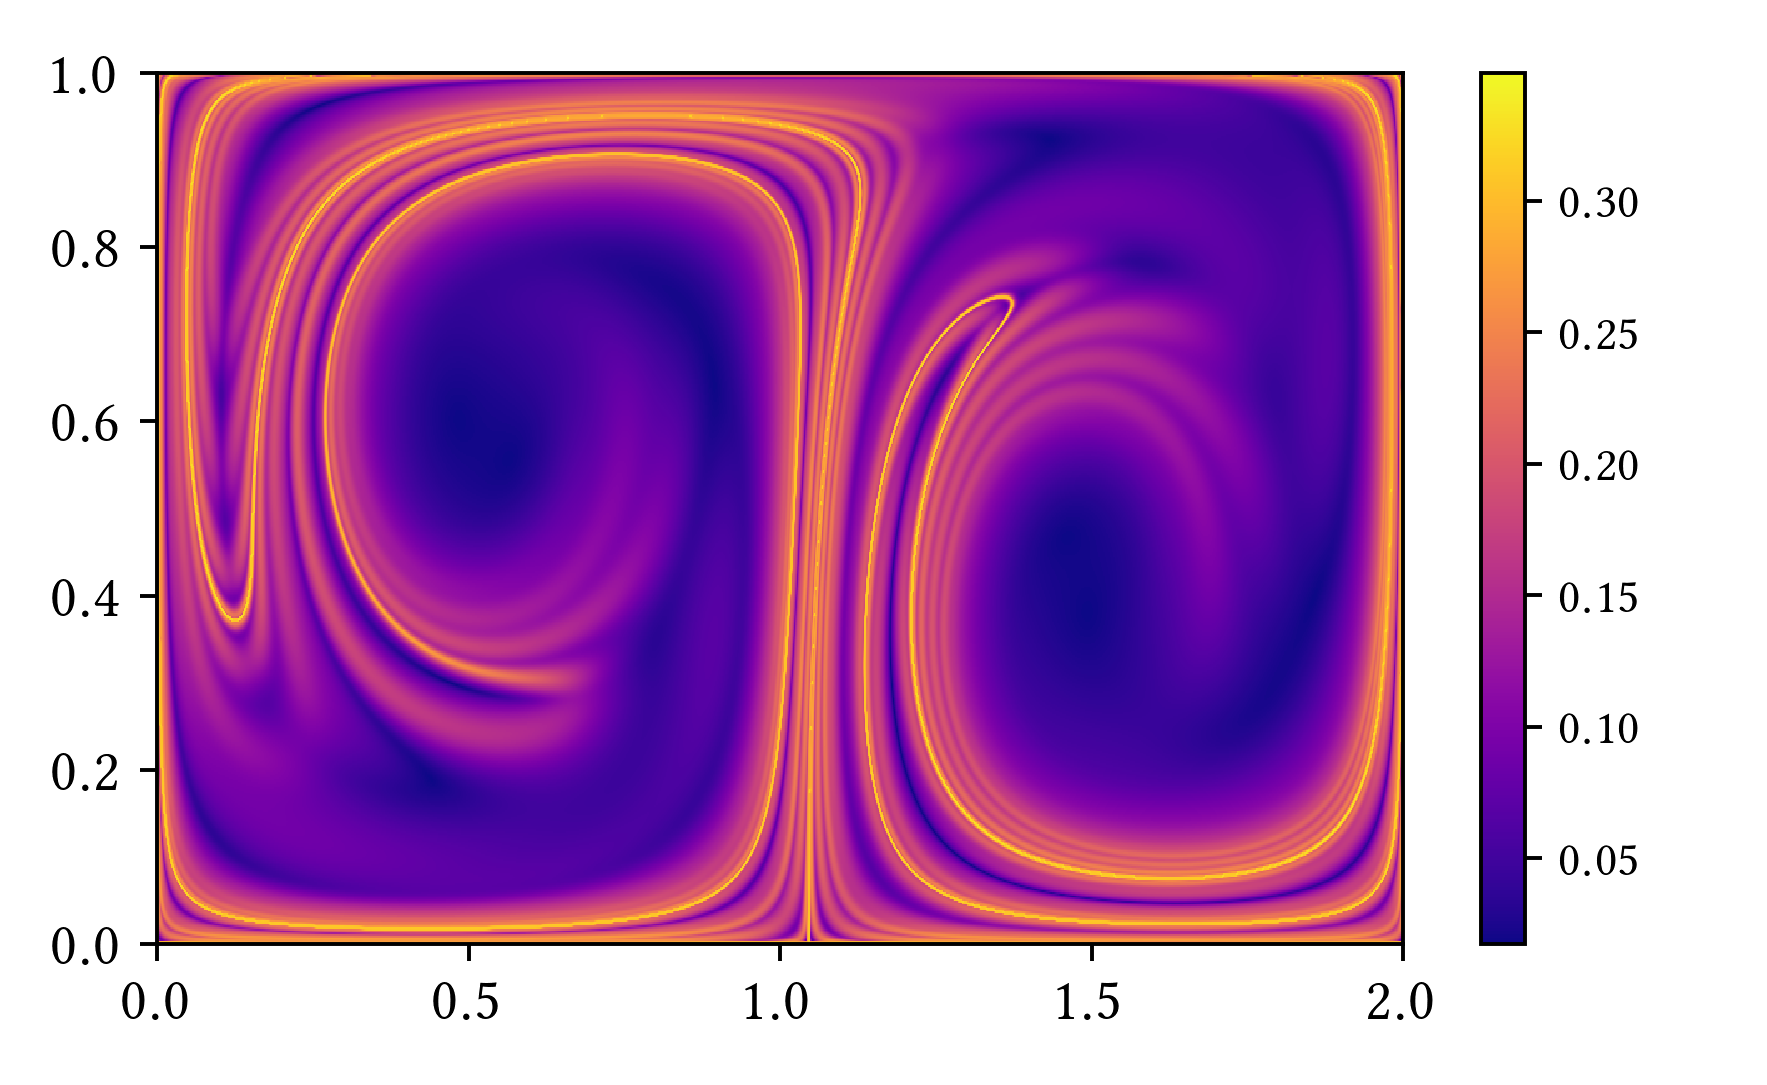
\includegraphics{figures/ftle_l2/ftle.png}
        \caption[]{FTLE field}
%        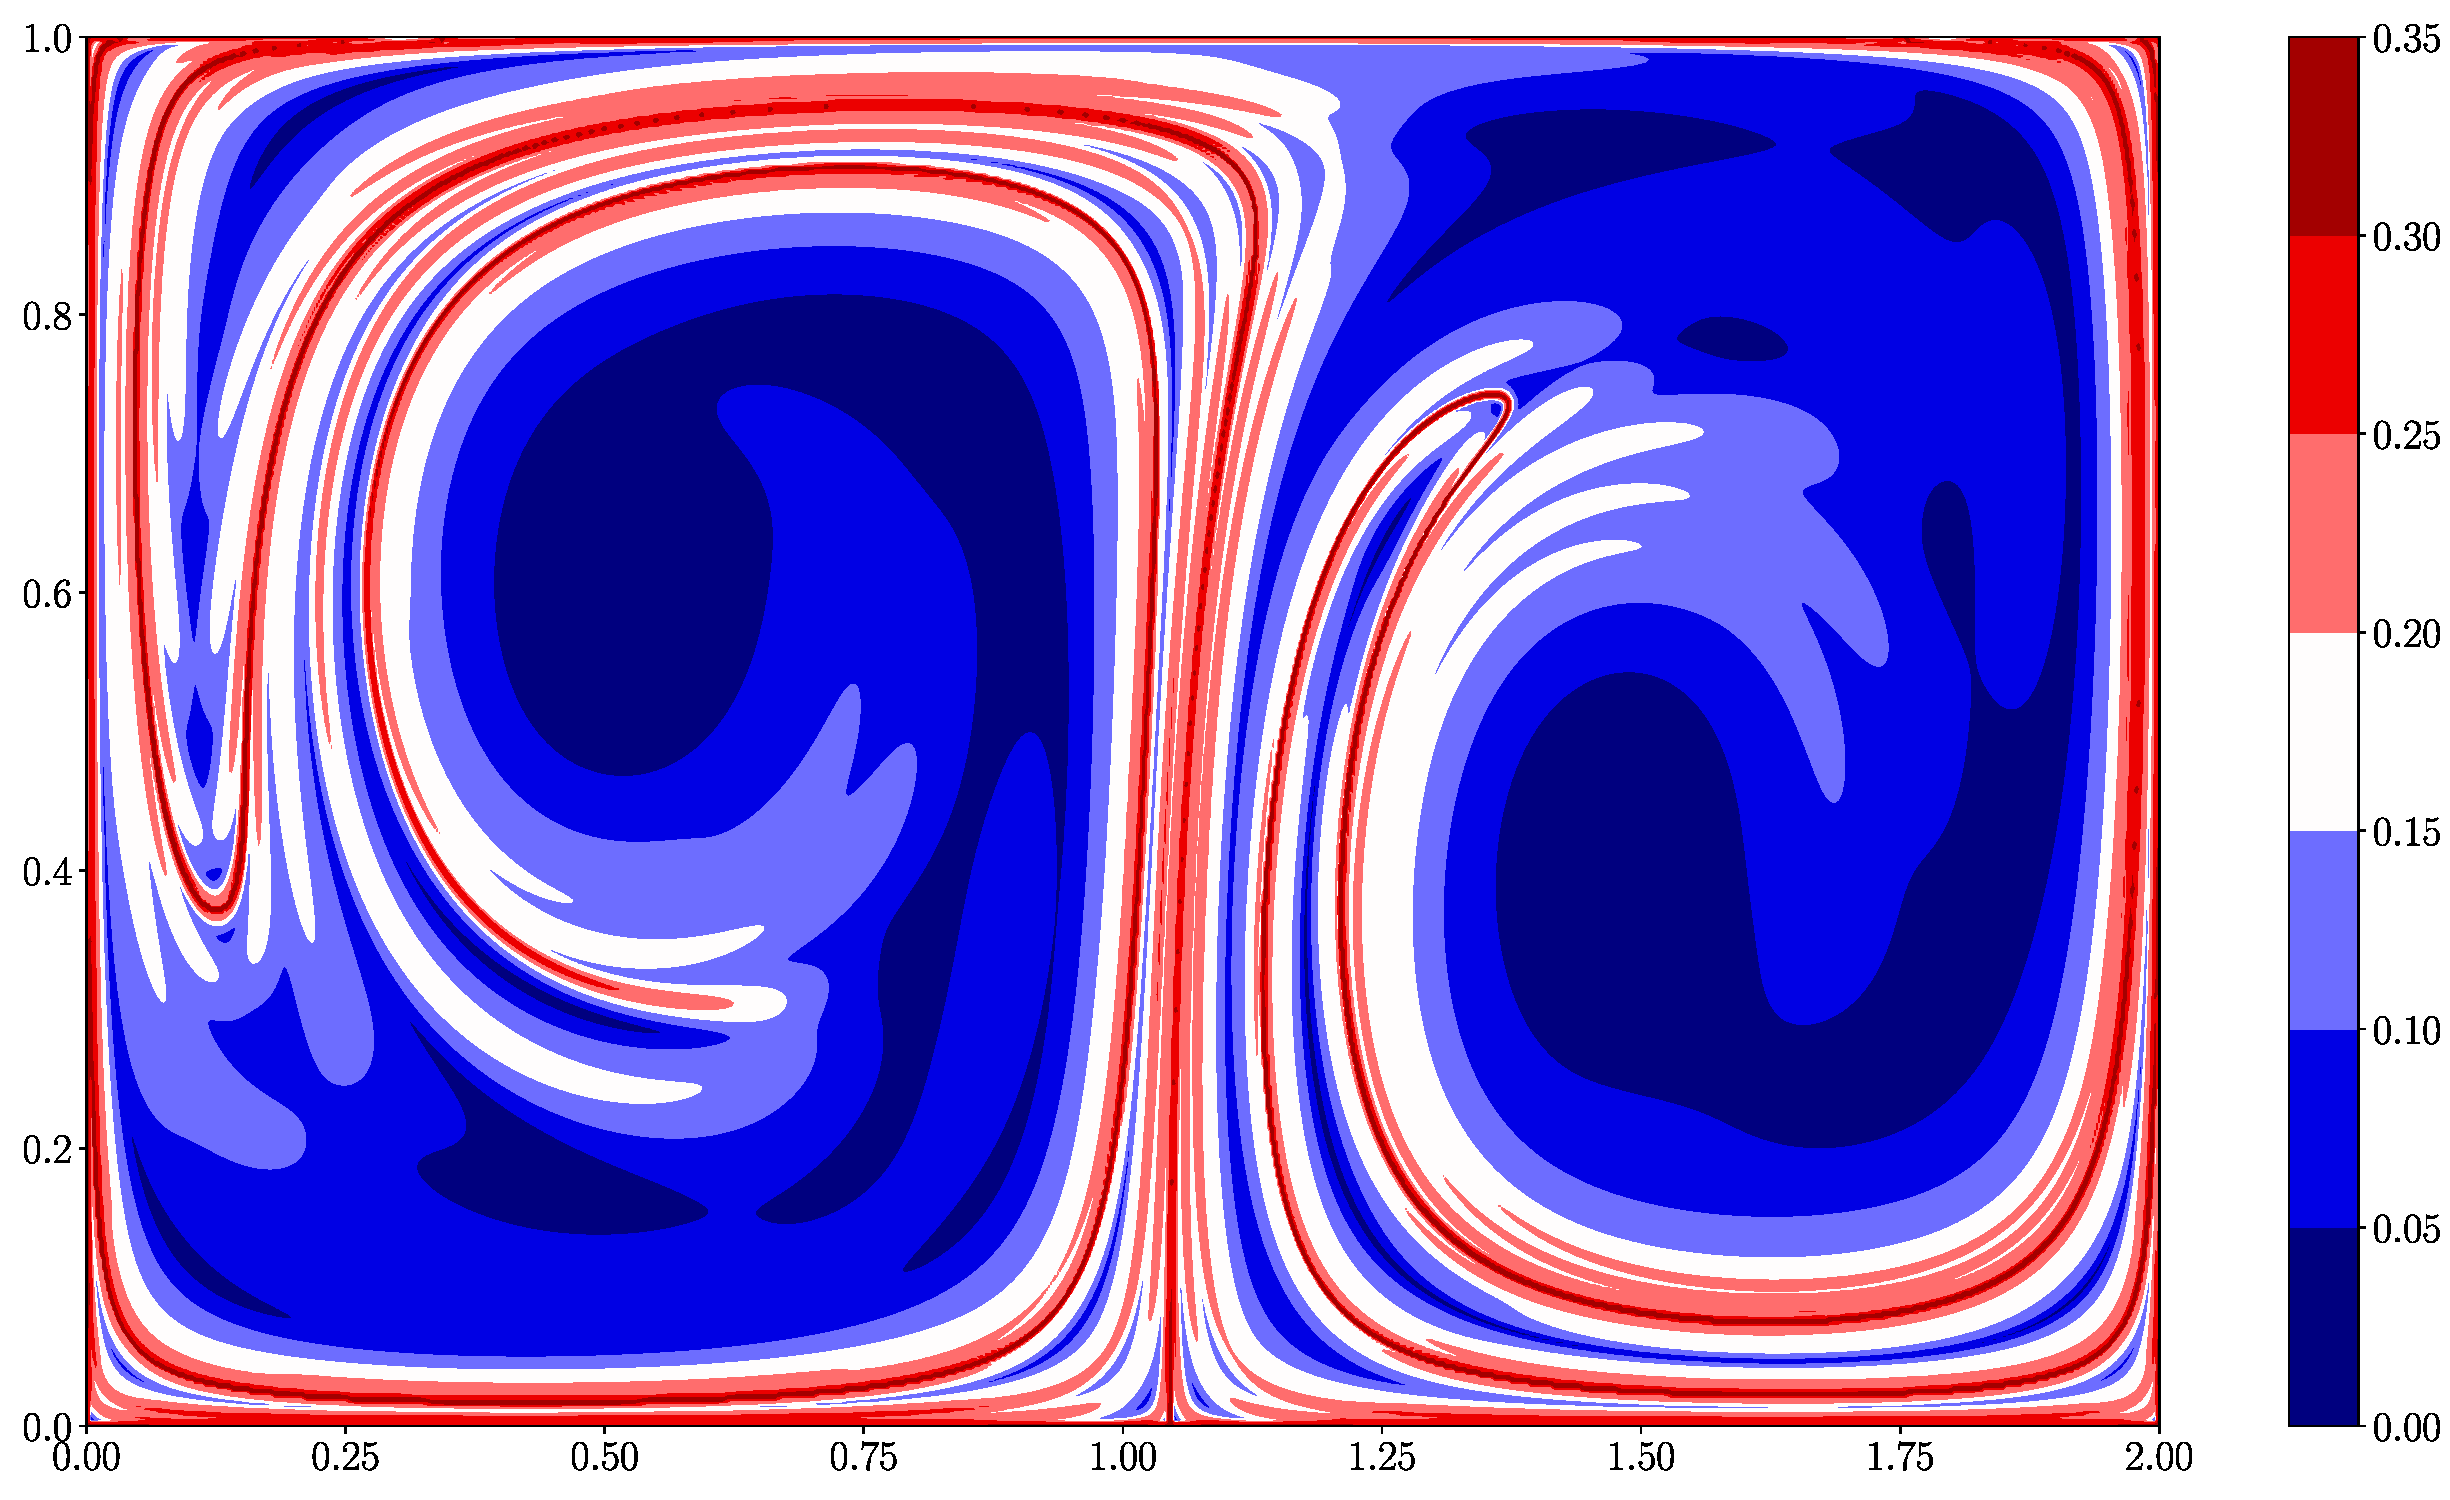
\includegraphics[width=0.75\linewidth,keepaspectratio]{figures/ftle.pdf}
        \label{fig:ftle_l2_ftle}
    \end{subfigure}

    \begin{subfigure}{\textwidth}
        \centering
        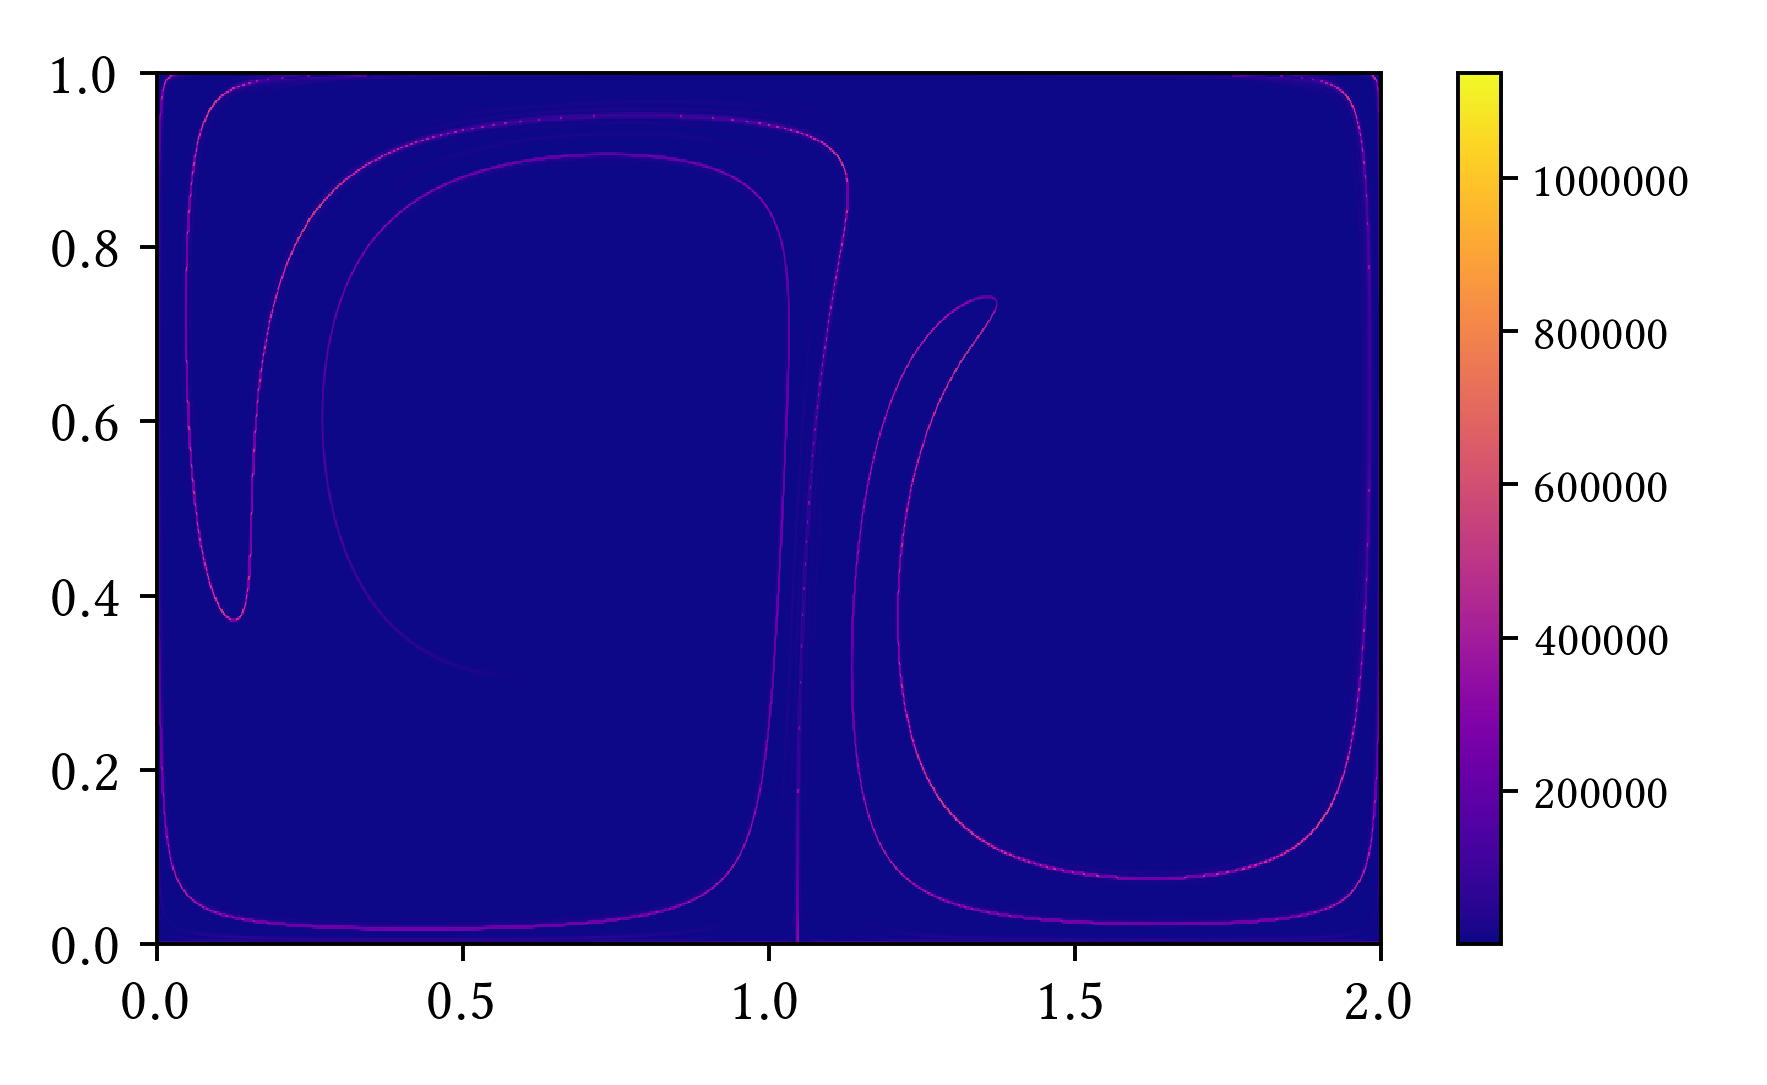
\includegraphics{figures/ftle_l2/l2.png}
        \caption[]{$\lambda_{2}(\vct{x}_{0})$ distribution}
        \label{fig:ftle_l2_l2}
%        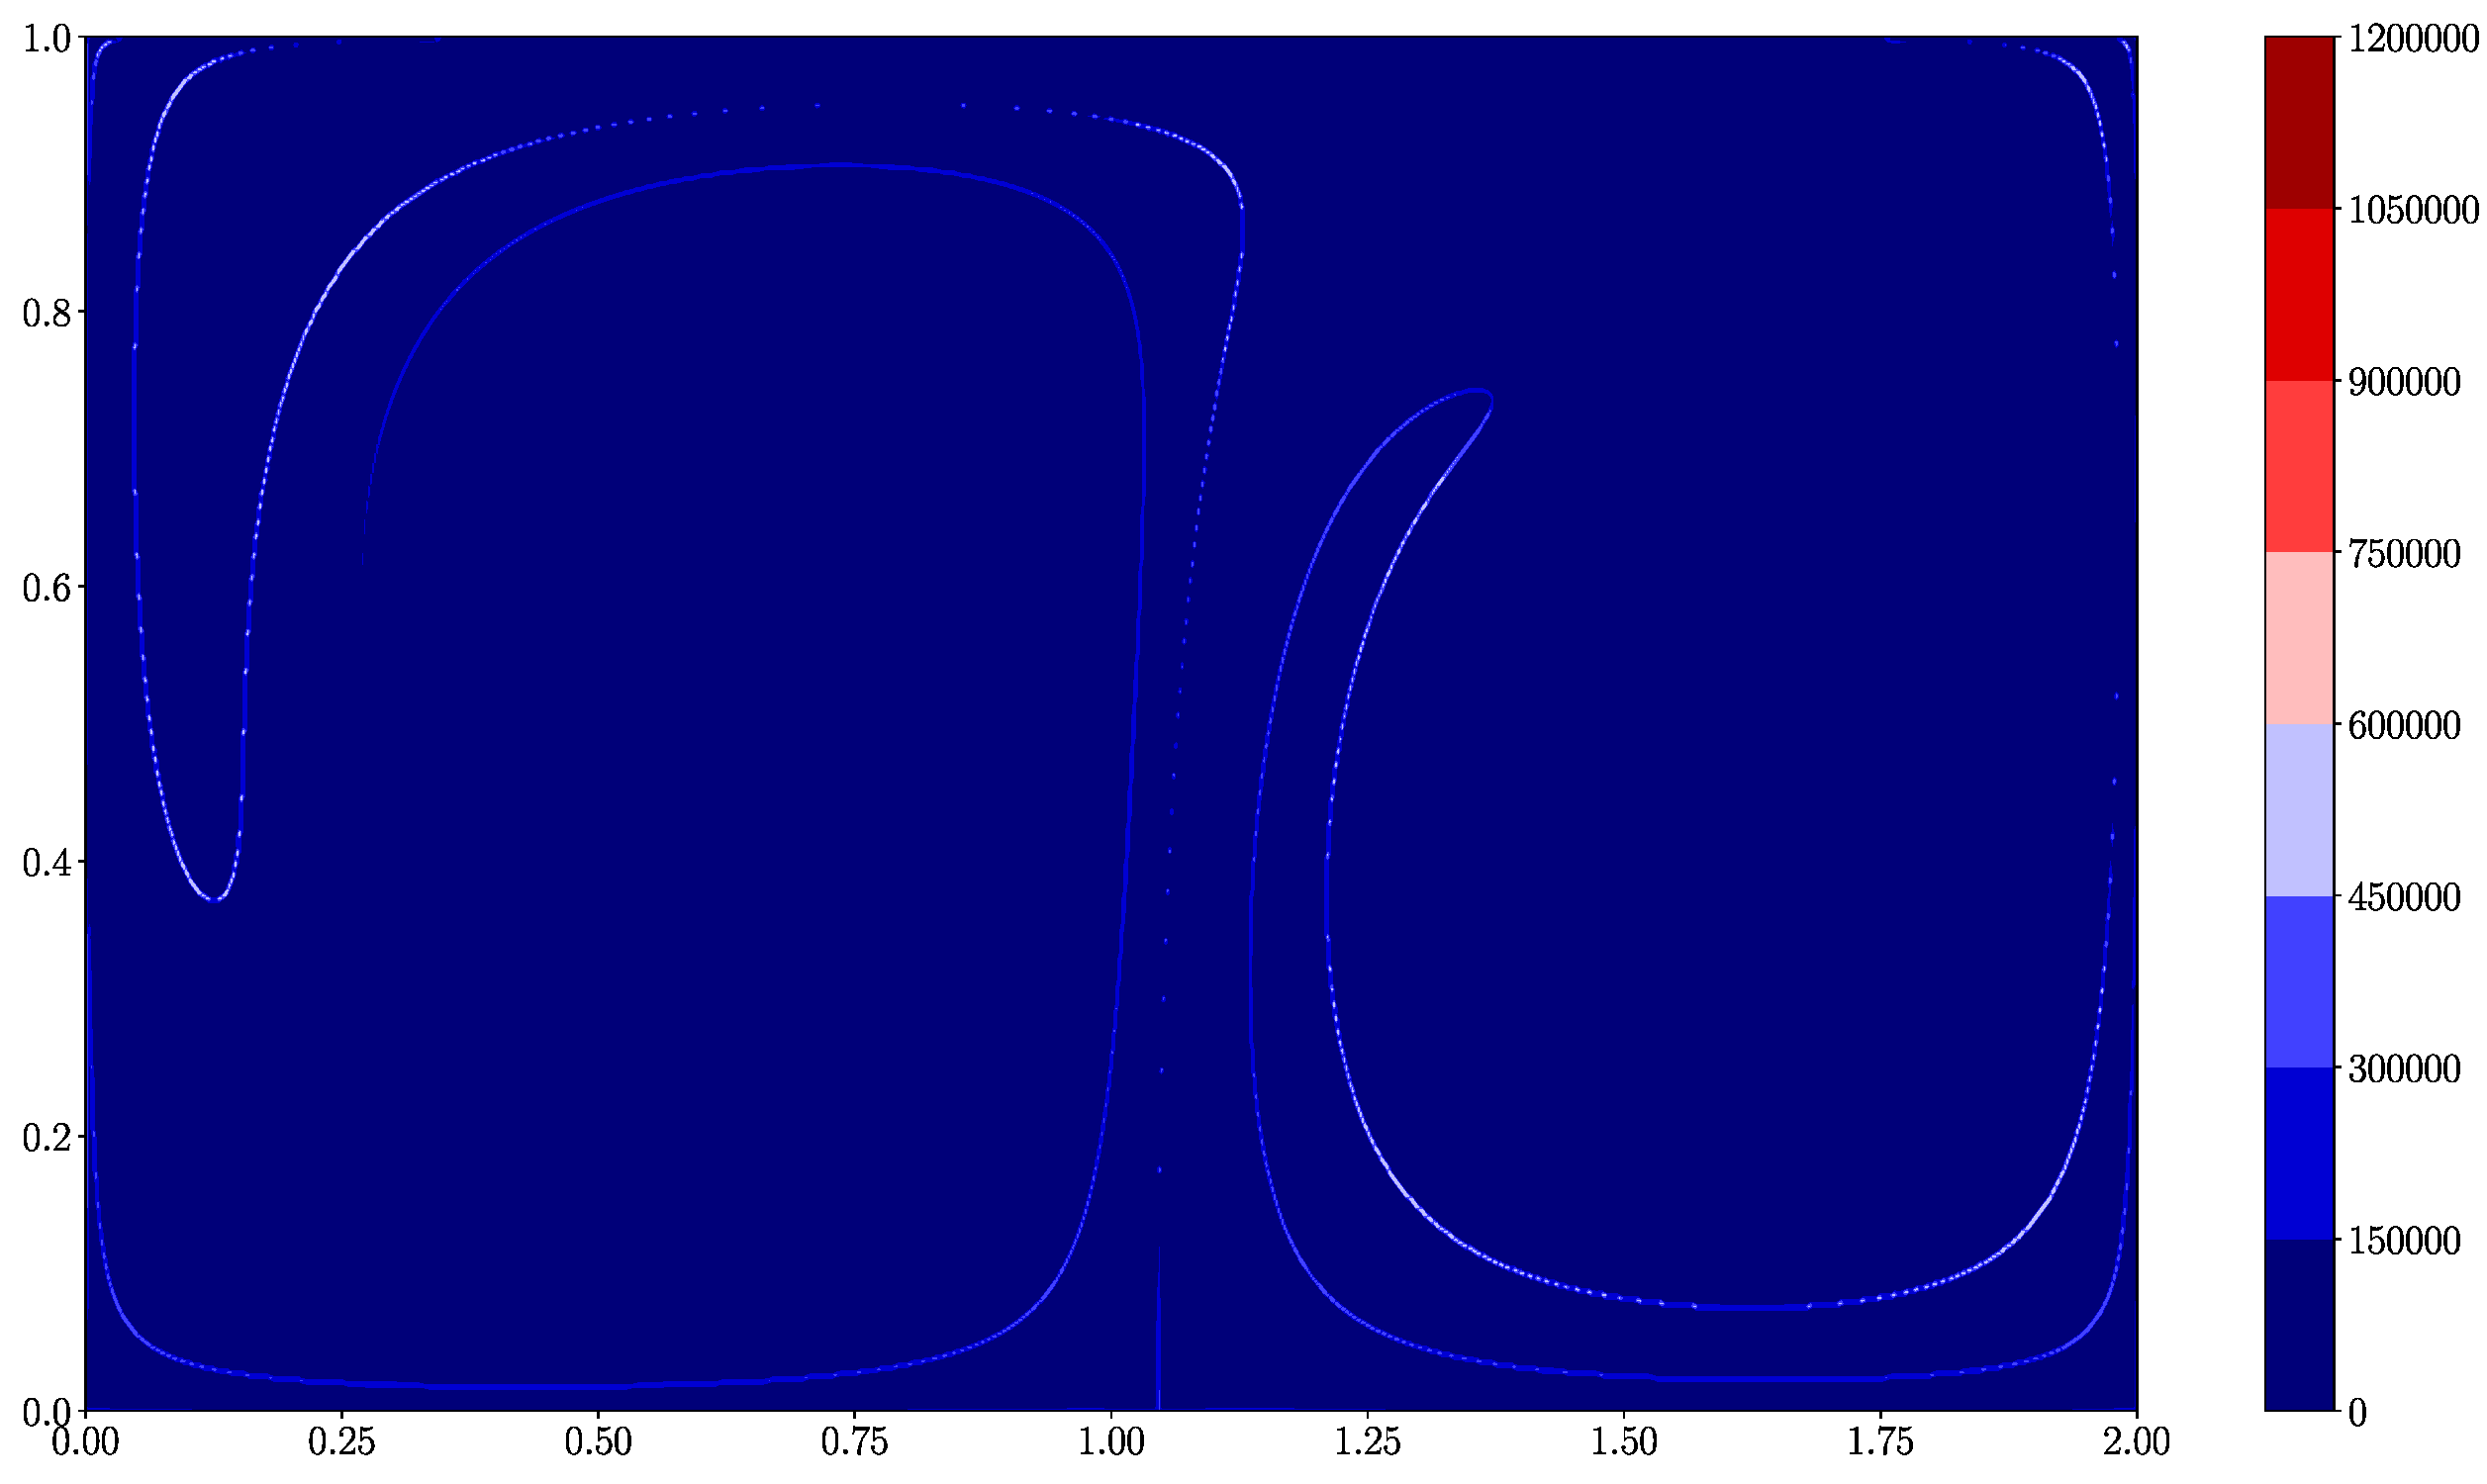
\includegraphics[width=0.75\linewidth,keepaspectratio]{figures/lambda2.pdf}
    \end{subfigure}
    \caption[Plots of the FTLE field and  $\lambda_{2}(\vct{x}_{0})$
    distribution of the double gyre system]{Plots of the FTLE field
    {(\subref{fig:ftle_l2_ftle})} and $\lambda_{2}(\vct{x}_{0})$ distribution
    {(\subref{fig:ftle_l2_l2})} of the double gyre system, given by equation
    \eqref{eq:doublegyre}. Due to the different scalings, different levels of
    detail are resolved. Most notably, the $\lambda_{2}(\vct{x}_{0})$ contains
    a thin, patchy ridge of extremal values, whereas a similar, albeit
    continuous structure is recognizable in the FTLE field. Moreover, the FTLE
    field exhibits a greater amount of detail away from the most prominent ridge
    than the $\lambda_{2}(\vct{x}_{0})$ distribution. Both contours were used,
    together with the domain $\mathcal{U}_{0}$ shown in figure
    \ref{fig:u0_domain}, in order to select the lines in $\mathcal{L}$,
    illustrated in figure~\ref{fig:neighborlcs}.
    }
    \label{fig:ftle_l2}
\end{figure}


\clearpage
The reference LCS, that is, the LCS obtained with the reference numerical
integrator, as mentioned in
\cref{sub:on_the_choice_of_numerical_step_lengths_and_tolerance_levels}, is
presented in figure~\ref{fig:referencelcs}. It consists of seven segments,
and agrees visually with the LCS found in the literature, for example by
\textcite{farazmand2012computing}. Note, however, that
\citeauthor{farazmand2012computing} claim that their LCS consists of a single
strainline segment. This will be elaborated upon in
\cref{cha:discussion}. The curve shown in figure~\ref{fig:referencelcs} was used to
benchmark how the different numerical integrators, mentioned in
\cref{sub:the_runge_kutta_methods_under_consideration}, for the parameters
mentioned in
\cref{sub:on_the_choice_of_numerical_step_lengths_and_tolerance_levels},
performed.

\begin{figure}[htpb]
    \centering
    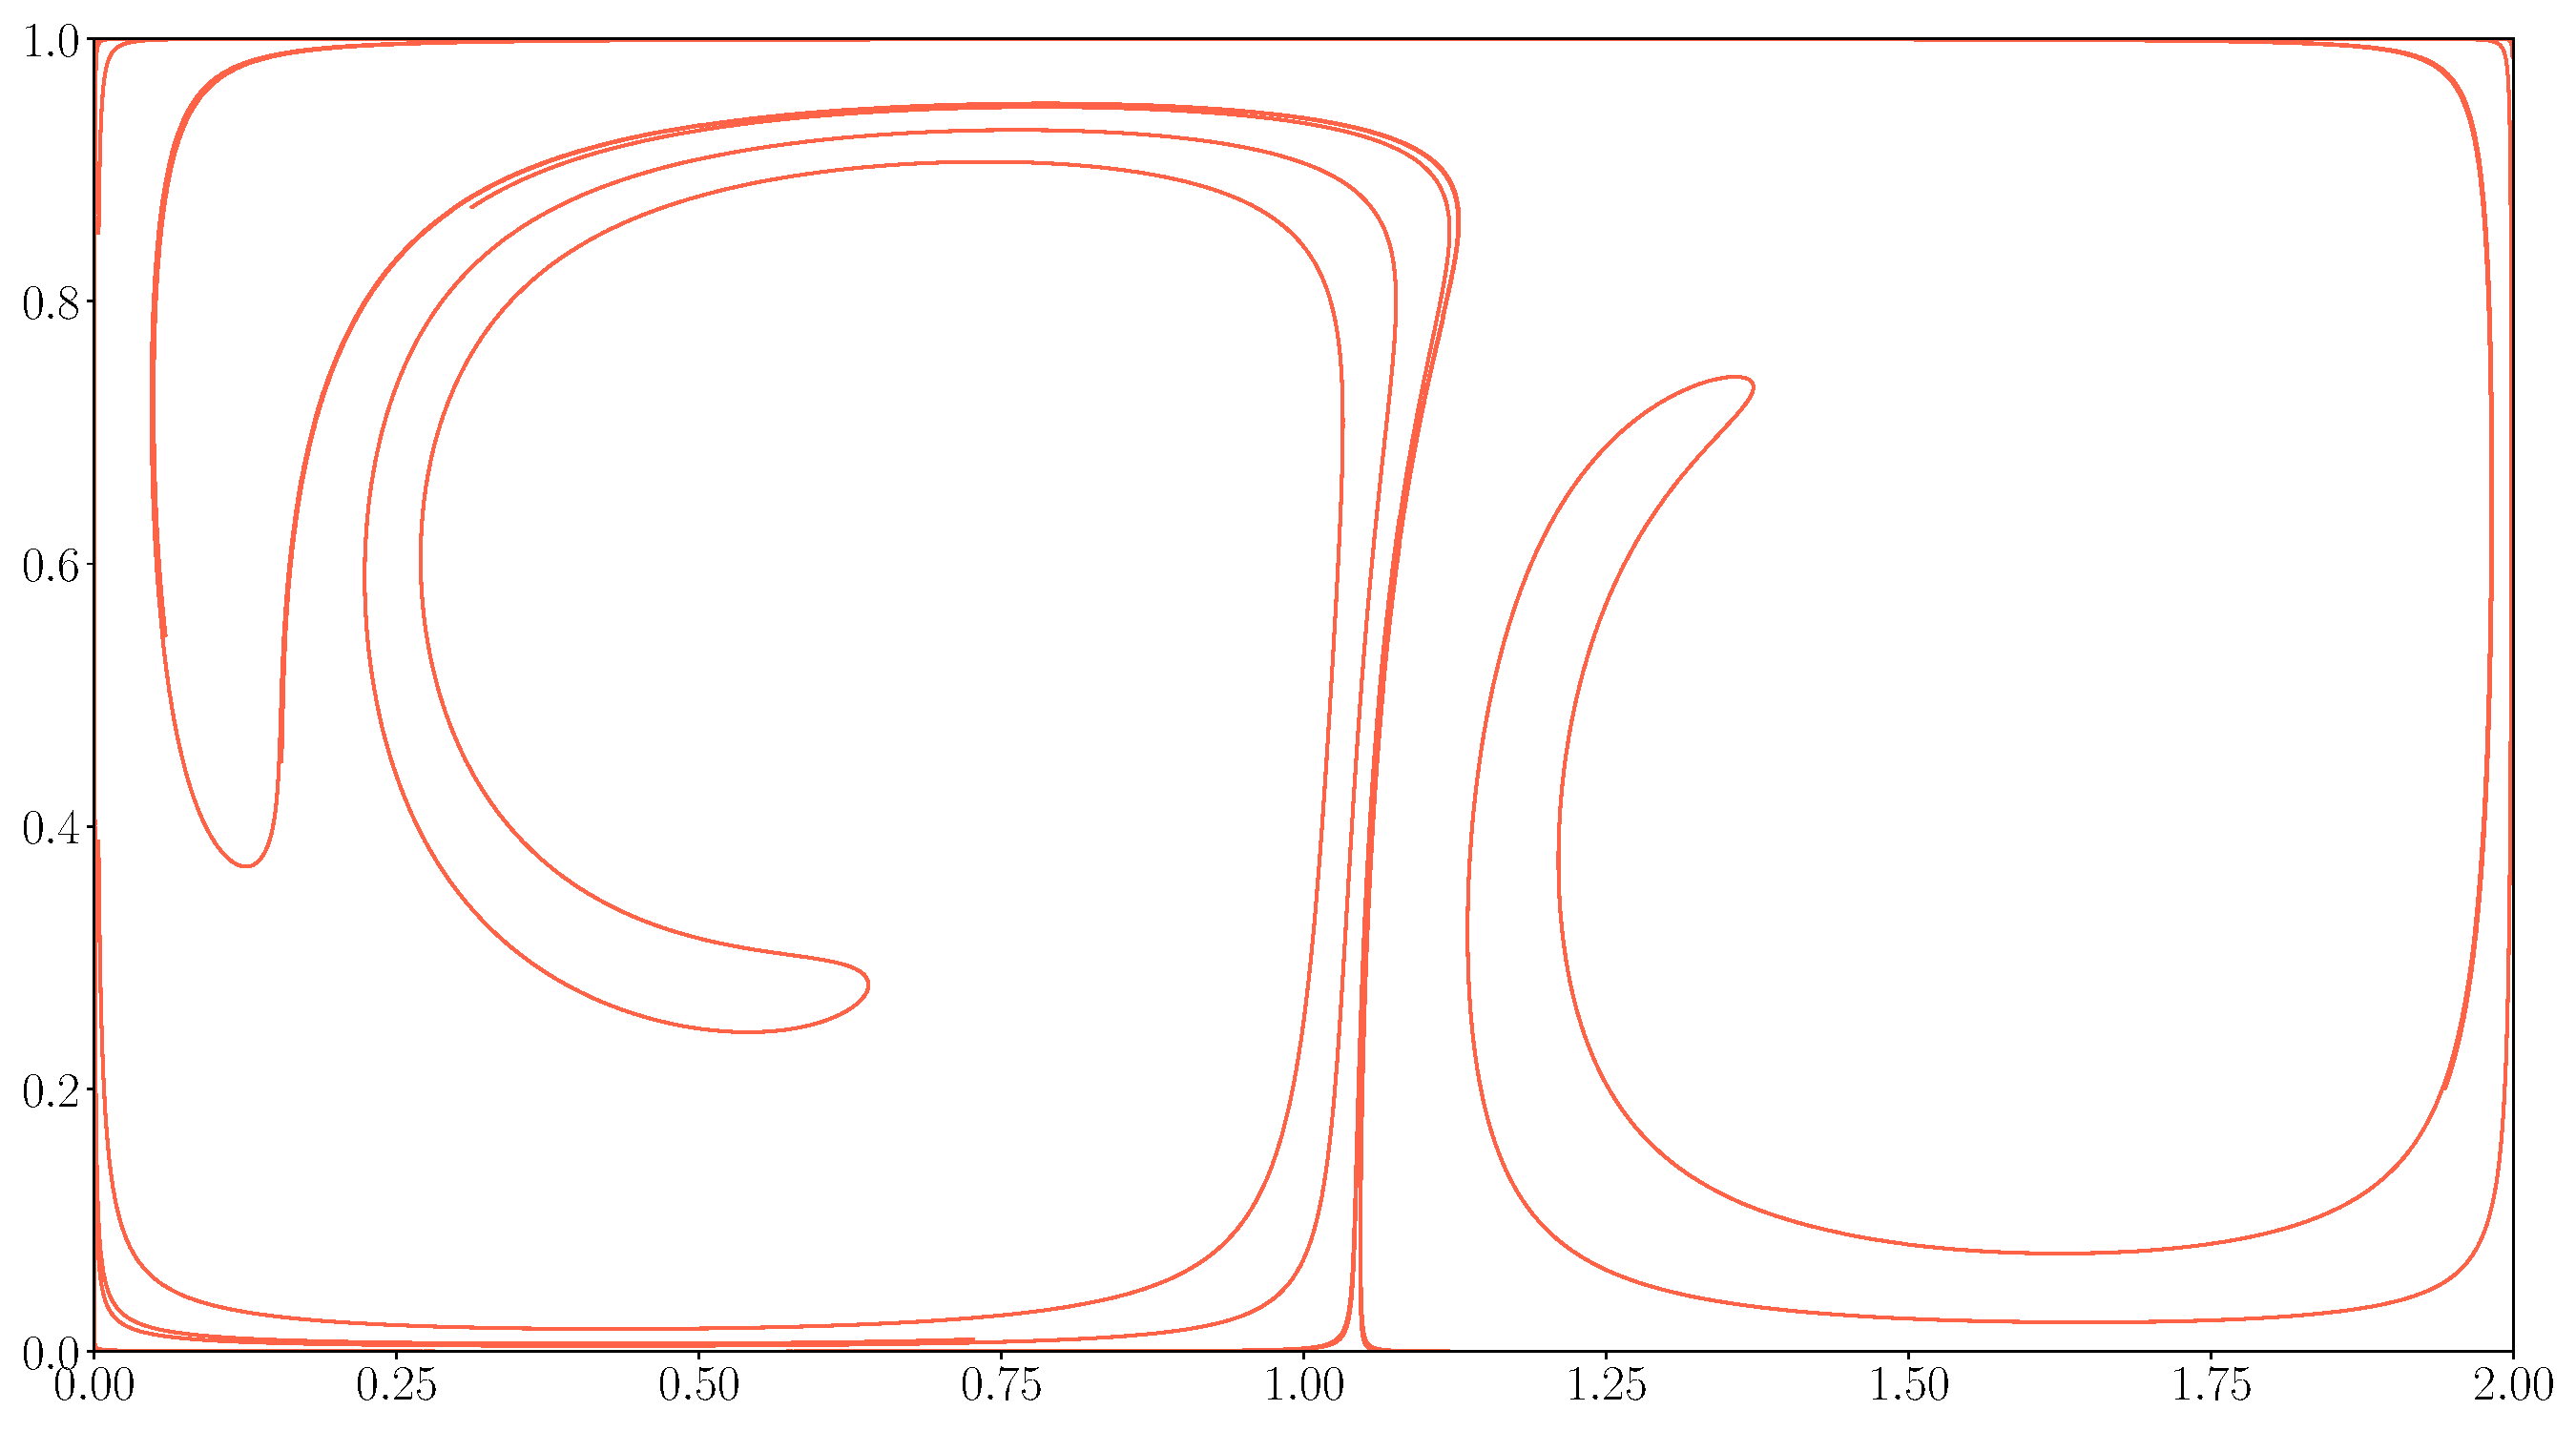
\includegraphics[width=0.9\linewidth]{figures/reference_lcs.pdf}
    \caption[The repelling reference LCS of the double gyre system]{The
    repelling reference LCS of the double gyre system, i.e., the LCS obtained
    by means of the reference numerical integrator, as outlined in
    \cref{sub:on_the_choice_of_numerical_step_lengths_and_tolerance_levels}.
    This curve agrees visually with the LCS found in the literature, for
    instance in \textcite{farazmand2012computing}. It was used as the benchmark
    for comparing the accuracy of the considered numerical integrators,
    outlined in \cref{sub:the_runge_kutta_methods_under_consideration}, for
    varying numerical step lengths and tolerance levels.}
    \label{fig:referencelcs}
\end{figure}




